\documentclass[a4paper,twoside,adobefonts]{ctexbook}
\usepackage[xetex,hidelinks,bookmarks]{hyperref}
\usepackage{ltxtable}
\usepackage{thesis}
\begin{document}


%前面几页不需要页眉页脚
\pagestyle{empty}

%封面
    \begin{titlepage}
	\begin{center}
		\noindent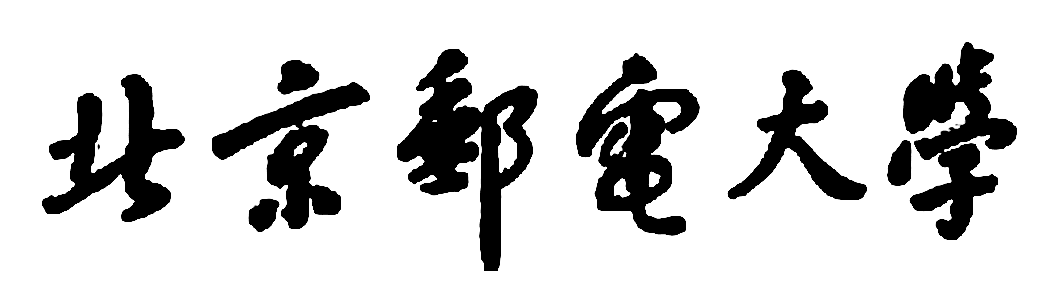
\includegraphics[height=2.5cm]{figures/spec/bupt_handwriting.eps}\\
		\vspace{4mm}	%本身有6.3mm的间隔
		\heiti\zihao{1}\textbf{本~科~毕~业~设~计~(论文)} \\
		\vspace{8mm}
		\noindent
\includegraphics[height=3.2cm]{figures/spec/bupt_logo.eps}\\
		\vspace{8mm}
		\setlength{\arrayrulewidth}{1pt}
		\begin{tabular}{@{}p{54.2pt}@{}p{233.4pt}}
      \heiti\zihao{3}\textbf{题目:} & \heiti\zihao{3}\hfill 基于MVVM架构的         \hfill \mbox{~} \\[-4pt] \cline{2-2}
			\heiti\zihao{3}\mbox{~}	      & \heiti\zihao{3}\hfill 课程管理系统设计与实现 \hfill \mbox{~} \\[-4pt] \cline{2-2}
		\end{tabular}\\
		\vspace{4mm}
    \begin{tabular}{@{}p{70pt}@{}p{180pt}@{}}
      \songti\zihao{3}\textbf{姓\qquad 名} & \songti\zihao{3}\hfill 陈杰      \hfill \mbox{~}\\[-4pt] \cline{2-2} %姓名
			\songti\zihao{3}\textbf{学\qquad 院} & \songti\zihao{3}\hfill 软件学院  \hfill \mbox{~}\\[-4pt] \cline{2-2}	%学院
			\songti\zihao{3}\textbf{专\qquad 业} & \songti\zihao{3}\hfill 软件工程  \hfill \mbox{~}\\[-4pt] \cline{2-2}	%专业
			\songti\zihao{3}\textbf{班\qquad 级} & \songti\zihao{3}\hfill 2010211501\hfill \mbox{~}\\[-4pt] \cline{2-2} %班级
			\songti\zihao{3}\textbf{学\qquad 号} & \songti\zihao{3}\hfill 10212043  \hfill \mbox{~}\\[-4pt] \cline{2-2}	%学号
			\songti\zihao{3}\textbf{班内序号}    & \songti\zihao{3}\hfill 11        \hfill \mbox{~}\\[-4pt] \cline{2-2}	%班内序号
			\songti\zihao{3}\textbf{指导教师}    & \songti\zihao{3}\hfill 刘禾      \hfill \mbox{~}\\[-4pt] \cline{2-2}	%指导教师
		\end{tabular}\\
		\vspace{12mm}
		\songti\zihao{3}\textbf{2014~年~6~月}
	\end{center}
\newpage
\rule{0pt}{0pt}
\newpage
    \end{titlepage}



%诚信声明
\begin{center}
\textbf{\songti\zihao{4}\ziju{1}北京邮电大学}  
\end{center}

\begin{center}
\textbf{\songti\zihao{4}\ziju{0} 本科毕业设计(论文)诚信声明}
\end{center}
\songti\zihao{-4}

本人声明所呈交的毕业设计(论文),题目《事件相关电位(ERPs)无线同步协议设计与系统实现》是本人在指导教师的指导下,独立进行研究工作所取得的成果。尽我所知,除了文中特别加以标注和致谢中所罗列的内容以外,论文中不包含其他人已经发表或撰写过的研究成果,也不包含为获得北京邮电大学或其他教育机构的学位或证书而使用过的材料。

申请学位论文与资料若有不实之处,本人承担一切相关责任。 \newline 

\indent 本人签名:\rule[-2pt]{4cm}{0.5pt}\quad 日期:\rule[-2pt]{4cm}{0.5pt}



%中文摘要
\newpage
\begin{center}
	\heiti\zihao{3}\textbf{基于 MVVM 架构的课程管理系统的设计与实现}
\end{center}
\begin{center}
	\heiti\zihao{-3}\textbf{摘\quad 要}
\end{center}
\vspace{2.5mm}
\songti\zihao{-4}

Model-View-ViewModel (MVVM) 模式是 Model-View-Controller (MVC) 模式的一种特例,2005 年由 Microsoft 提出并首次应用于 Windows Presentation Framework (WPF),MVVM 模式将 MVC 架构模式与 Observer 模式配合使用,在 Model、ViewModel 与 View 之间通过 DataBinding 建立关系,解决了图形用户界面(Graphical User Interface)开发中对异步事件处理的难点,近年来十分受到业界的重视。

本文以课程管理系统的设计与实现为例,对比分析 MVVM 模式的开发性能,同时尝试对 MVVM 模式在 JavaScript 语言平台上的实现提出改进方案。借助 JavaScript 语言平台支持函数式编程的特性,在 MVVM 框架中引入 Functional Reactive Programming (FRP) 的设计思想,并从 Reactive Programming 的角度分析讨论 MVVM 模式在处理异步逻辑方面的优越性、设计基于 Monad 对象实现 ViewModel 的改进框架。

\vspace{3mm}
\zihao{-4}\heiti\textbf{关键字}\quad \songti MVVM \quad 富应用 \quad Reactive Programming \quad 课程管理系统



%英文摘要
\begin{center}
\zihao{3}\textbf{An MVVM Based Course Management System}
\end{center}
\begin{center}
\zihao{-3}\textbf{ABSTRACT}
\end{center}
\vspace{2mm}
\zihao{-4}

Model-View-ViewModel (MVVM) design pattern is a pattern providing a resolution to asynchronous programming of Graphical User Interface (GUI) which is introduced into Windows Presentation Framework (WPF) at 2005 by Microsoft. Based on Observer Pattern, MVVM uses feature called DataBinding to make connection between Model, ViewModel and View objects. With it's success in handling asynchronous events, MVVM has been adopted widely Rich Interaction Applications (RIAs).

The subject of this article is to design a Course Management system based on MVVM framework, and, introduce improvement to MVVM development on JavaScript platform.

A typical Object-oriented MVVM implementation on JavaScript platform does not make use of functional programming ability of JavaScript. The article tries to introduce the idea of Functional Reactive Programming (FRP) into MVVM design and analyse the use of Observer in typical MVVM implementation from the view of Functional Programming Language. Then, bring up the ViewModel built by Monad objects.

\vspace{3mm}
\zihao{-4}{\bfseries KEY WORDS}\quad MVVM \quad FRP \quad Asynchronous Programming \quad Management System


\frontmatter{Roman} %开始罗马页数计数

%目录
\tableofcontents

\mainmatter	%开始阿拉伯数字计页数

%从正文开始加入页眉和页脚
\pagestyle{fancy}

%正文
\chapter{概述}

本章介绍课程管理系统的项目背景并简要阐述 Model-View-ViewModel (MVVM) 模式、Functional Reactive Programming (FRP) 方法的核心思想及特性。

\section{项目背景}

用户交互(User Interaction)在消费级产品开发中的地位近年来正不断提升,交互设计和实现正成为产品开发中最重要也最复杂的环节之一。随着互联网的发展、富交互应用(Rich Interaction Application, RIA)的兴起,交互设计正走向越来越复杂的方向。使用传统的命令式编程(Imperative Programming)实现用户交互逻辑的局限性也不断显现出来。

Microsoft 在 Windows Presentation Framework (WPF) 中引入的 Model-View-ViewModel(MVVM) 模式近年来得到了相当广泛的关注和应用~\footnote{Wikipedia: Model View ViewModel}。MVVM模式作为如今最成功的图形用户界面(Graphical User Interface, GUI)开发模式之一,将声明式方法引入用户交互开发,解决了命令式编程方法在处理异步逻辑时难于维持代码逻辑连续性的问题。

课程管理系统作为面向业务产品的典型代表,工程规模足够体现设计模式的各项性能。本文以课程管理产品的设计与开发为线索,尝试解释 MVVM 设计模式的设计方法,并从 FRP 的角度解释 MVVM 模式中 ViewModel 部分的设计,在此基础上使用 monad 结构~\cite{raey}开发 MVVM 框架并测试该框架在课程管理系统中实际进行富交互应用开发的性能。

\section{Model-View-ViewModel~模式}

经典的 MVC 模式~\footnote{Wikipedia: Model–view–controller} 将系统分成 Model(模型)、View(视图)、Controller(控制器) 三个部分: Model 对象用于处理数据和业务操作、View 对象控制视图逻辑、Controller 负责处理用户操作。MVC 架构作为许多互联网产品和应用的基础架构在各大开发平台都有成熟的解决方案和技术框架~\footnote{如 Ruby-on-Rails、ThinkMVC 等广泛应用的 Web 框架都基于 MVC 架构进行开发}。

\begin{figure}[!h]
\begin{center}
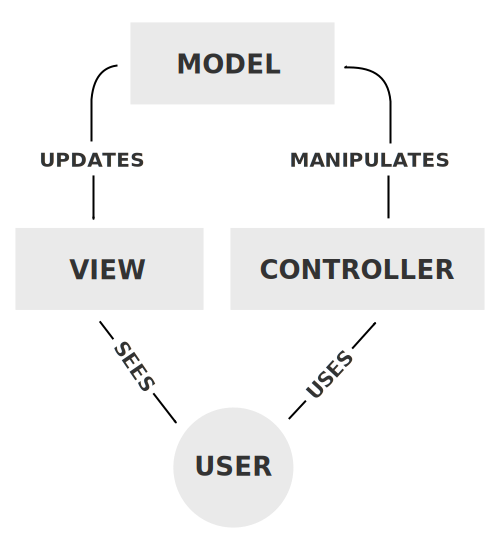
\includegraphics[scale=0.5]{figures/MVC-Process.pdf}
\caption{MVC 模式\label{MVCOverview}}
\end{center}
\end{figure}

Microsoft 作为用户交互领域的先驱,最早在 2005 年由工程师 Martin Fowler 提出了 MVVM 架构并应用于 Windows Presentation Framework。

\begin{figure}[!h]
\begin{center}
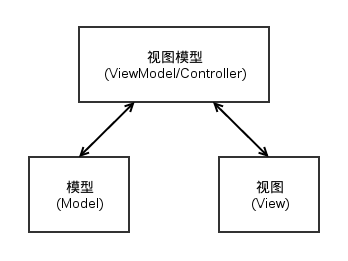
\includegraphics[scale=0.7]{figures/MVVMOverview.png}
\caption{MVVM 模式\label{MVVMOverview}}
\end{center}
\end{figure}

Model-View-ViewModel (MVVM) 模式是 Model-View-Controller (MVC) 模式的一种特化(见图~\ref{MVVMOverview}): MVC 模式中 Controller 负责进行的界面业务逻辑部分抽象为 ViewModel 以及 Binder 组合。一方面利用 ViewModel 管理交互状态、另一方面通过 Binder 将状态通过 View 进行展示。用户产生的交互事件也经由 Binder 传递至 ViewModel 对用户界面的状态以及 Model 状态产生影响。

MVVM 模式的一大设计亮点在于“ViewModel 继承于 Model” 即: ViewModel 可以将另一个 ViewModel 实例作为 Model 进行数据请求。这是 ViewModel 与 Controller 之间最大的不同,也是 ViewModel 较 Controller 实现拥有更高的可复用性以及更良好的可测试性的原因。

另外,MVVM 模式解除了 Controller 代码与视图实现之间的耦合关系,界面设计人员仅需要在XAML(对WPF的情况)文档中描述视图对象所需要绑定(bind)的数据位置(属性名称)即可完成用户交互设计任务,而在 MVC 模式中设计者需要书写 Controller 代码以描述视图对象所需要的呈现数据。

MVVM 模式在普遍用于用户交互开发的 JavaScript 语言中也得到了类似的实现,如 AngularJS、KnockoutJS 等开发框架。

\section{Functional Reactive Programming (FRP)}

Functional Reactive Programming (FRP) 是使用声明式 (Declarative) 方法描述系统行为的编程方法。FRP 的主要思想是将系统抽象为 $行为(Behaviors)$ 和 $事件(Events)$,使用行为表示系统中随时域连续变化的值、事件表示一系列按一定时序触发的离散值~\cite{Wan:2000:FRP:358438.349331}。最初,FRP 方法被应用于 Haskell 的 Functional Reactive Animation (Fran) 的核心实现~\cite{Elliott:1997:FRA:258949.258973}。后来,FRP 方法被广泛的用于计算机视觉、机器人以及其他控制系统的设计和实现。

简而言之,FRP 抽象系统为用户与函数(Behavior)的交互,用户事件作为函数的自变量,而模型/用户视图作为函数作用的因变量。

随着 FRP 理论的成熟与富交互应用的发展,FRP 的影响也逐渐延伸到应用开发的前沿领域,出现了许多成熟的 FRP 开发框架,如 Objective C 平台下的 ReactiveCocoa,.NET Framework 下的 ReactiveUI 以及 JavaScript 平台下的 Reactive.js 等~\footnote{虽然这些框架是实现在命令式语言平台的 Reactive Programming 框架,这里还是沿用 Haskell 中 FRP 的名称}。

FRP 方法与 MVVM 使用的 Observer 模式具有很高的相似性,本文将在后面的章节围绕此问题进行一番讨论并提出作者对 MVVM 架构模式的理解。

后文分成五个部分: 第二章、第三章分别介绍系统的需求分析和概要设计,第四章引入有关MVVM模式与 Reactive Programming 的讨论、描述 ReactiveVM 的设计思路,第五章讨论实现过程中出现的探索性过程,第六章对项目的开发过程进行一个总结并描述一下对未来研究方向的展望。


\chapter{方法-协议设计\label{chp:protocol}}
本章主要介绍了事件相关电位无线同步的协议设计,主要思想是通过子钟硬同步对准避开无线传输延迟的影响,误差主要取决于系统提供时钟信号的晶振偏差;同时协议还兼容了无线脑电放大器~\cite{Xu2009}的数据格式,并新增加了一个数据包结构用于传输自适应参数。
\section{基本思路-子钟对准硬同步}
\subsection{子钟概念引出}
在卫星发射等航天任务中也需要子钟,以地球同步轨道卫星发射为例,如图~\ref{GeostationarySate},卫星在升空进入椭圆轨道后在距离地球36000千米处加速进入地球同步轨道,以光速计算这个传输的延迟是:
\begin{equation}
\frac{36000 \times 10^{3}}{3 \times 10^{8}} = 0.12 s  
\end{equation}

即地球站给卫星的信号需要经过至少0.12s的传输才能被卫星接收到。再考虑由于距离远,无线数据传输出错需要纠正重发,卫星收到数据后需要向地面确认收到信号等因素,实际完成通信时间会远远大于0.12s,如果地面对于卫星的控制采用卫星实时接收数据并执行的方式,那么可以想见,卫星就不可能准确的进入地球同步静止轨道。

\begin{figure}[!hbp]
\begin{center}
\includegraphics[width=\textwidth]{graphic/GeostaiontarySatellite.PNG}
\caption{ 地球同步卫星发射轨道 \label{GeostationarySate}}
[卫星从地球发射后会进入绕地椭圆轨道(如图中椭圆所示),在达到距地最远点时点火加速脱离椭圆轨道进入地球同步轨道]
\end{center}
\end{figure}

实际采取的措施是:卫星携带一个振荡偏差小于$10^{-14}$的原子钟,在升空之前先与地面原子钟完成对时,升空后地面对卫星的控制通过提前发送控制信号给卫星,指定以几点几时几分几秒时执行某种指定操作,从而大大提高了卫星执行操作的时间准确性。

把这一概念运用到刺激事件与EEG脑电的同步中,设计了如图~\ref{WirelessTriggerSche}所示的系统,对比图~\ref{WiredBCI}可见,系统增加了一个无线同步触发器(Wireless Trigger)来接收EEG脑电数据和刺激事件信号(Marker Code),数据在无线同步触发器上完成同步以后返回给计算机。由图~\ref{WirelessTriggerSche}可见被试只需要头戴电极帽并携带脑电放大器(EEG Amplifier),数据通过无线发送给无线同步触发器,简化了用户端的连接。无线同步触发器的具体实现在\quad 第三章~系统实现\quad 中讨论。

\begin{figure}[!hbp]
\begin{center}
\includegraphics[width=\textwidth]{graphic/SubClockWirelessSch.PNG} 
\caption{ 基于ERP无线同步协议的脑机接口系统原理图 \label{WirelessTriggerSche}}
\end{center}
\end{figure}

\section{子钟同步过程}
数据传输之前,无线同步触发器与脑电放大器先进行子钟对准,使其各自的内部计数器以相同的起始值和相同的时间间隔递增。同步之前先需要进行握手以确认连接。整个子钟同步的过程可以分为:握手,使能计数器,同步确定三个步骤。
\subsection{三次握手}
	握手过程采用了有线连接以减少传输延迟并提高对准的精度。同步双方(这里是脑电放大器和无线同步触发器)各设置两个IO口分别为同步输入和同步输出端。然后按图~\ref{handshankeHard}所示的方式连接,即脑电放大器同步输出接无线同步触发器同步输入,无线同步触发器同步输出接脑电放大器同步输入,另外还需要将两个设备共同接地以防止基准电平的不同。

\begin{figure}[!hbp]
\begin{center}
\includegraphics[width=\textwidth]{graphic/ConnectionSynchronization.PNG}
\caption{ 同步握手连接图 \label{handshankeHard}}
\end{center}
\end{figure}

握手过程时序如图~\ref{TFHardwareSyn}所示:图中用A和B代表同步双方,A\_{}O表示A的输出端口,A\_{}I表示输入端口,B类似。

\begin{figure}[!hbp]
\begin{center}
\includegraphics[width=\textwidth]{graphic/TimeFlowHardwareSynch.PNG}
\caption{ 硬件握手时序 \label{TFHardwareSyn}}
[横轴为时间轴]
\end{center}
\end{figure}

握手过程描述如下:
\begin{enumerate}
\item 初始化端口状态,A的输出初始化设置为高电平,表示为A\_{}O = 1;相应的B\_{}O = 0;
\item 延时一段时间;(实际测试中发现,如果初始化完成后立即开始检测输入电平,由于两边系统初始化时间不同,一边开始检测端口状态时,另一方可能尚未初始化端口电平,而端口输出状态不可控,导致握手失败。)
\item	A,B输入端口开始检测输入电平;
\item B输入首先检测到高电平,如图~\ref{TFHardwareSyn} 中B\_{}I行第一个 {\textcircled{\small{1}}} (B\_I = 1);随后B置高其输出端口(B\_O = 1);并重新开始检测其输入端电平(B\_I == 0?)。
\item 输入在检测到端口电平抬高(A\_{}I = 1),如图中第二个 {\textcircled{\small{1}}}; 置低其输出端(A\_{}O = 0)并重新检测输入(A\_{}I == 0?);
\item 上一步A的操作导致B的输入端置低 (B\_{}I = 0),如图~\ref{TFHardwareSyn} B\_{}I 行的 {\textcircled{\small{2}}},随后B也将输出置低 (B\_{}O = 0);
\item A输入端检测到置低,然后A输出置高,第三次握手的过程类似上面的描述。
\end{enumerate}

	两边都完成是三次的握手以后就相互确认了连接状态。最后一个完成握手的A在第三次确认输入置高以后,延迟100ms以便同步的另一方B能有时间做好同步前的准备,A设置相关计数器的初始值,然后再次给出一个低电平并将己方的\textbf{同步计数器使能},B在检测到电平翻转以后也同时使能计数。由于有线连接的延迟基本上可以忽略不计,同步双方完成同步计数。
%图~\ref{SynWaveLarScale}展示了两个系统同步时的电平对准,从图~\ref{SynWaveSamScale}
%
%\begin{figure}[!hbp]
%\begin{center}
%\includegraphics[scale = 0.5]{graphic/05312010479.jpg}
%\caption{ 脑电放大器与无线同步触发器同步时刻波形(大) \label{SynWaveLarScale}}
%\end{center}
%\end{figure}
%
%\begin{figure}[!hbp]
%\begin{center}
%\includegraphics[scale = 0.5]{graphic/05312010478.jpg}
%\caption{ 脑电放大器与无线同步触发器同步时刻波形(微) \label{SynWaveSamScale}}
%[上波形为主动发动同步的无线同步触发器,下波形为检测到无线同步触发器上升沿以后也开始同步的放大器输出波形,可以看到初始延迟为一个上升沿的时间,5$\mu$s]
%\end{center}
%\end{figure}
%
	采用三次握手可以避免一些如图~\ref{noiseDigital}所示的错误信号。

\begin{figure}[!hbp]
\begin{center}
\includegraphics[width=\textwidth]{graphic/10.PNG}
\caption{ 常见数字干扰波形图 \label{noiseDigital}}
\end{center}
\end{figure}

\subsection{同步确认}
由于本系统中的脑电放大器和无线同步触发器还通过无线方式连接,一方面在数据传输前最好能确认无线连接已经建立,另一方面虽然三次握手避免了误同步操作,但是同步的双方终究还是不知道对方的情况,比如A同步了但是B没有同步。由于A是同步发起方,因此在双方完成同步以后令B给A通过无线发送一个信号表明自己确实也完成同步了。这样既确认了无线连接,又确认了双方都已经同步。

\section{数据传输格式与兼容性}
	从图~\ref{WirelessTriggerSche}可知,数据传输涉及到三个设备:脑电放大器,无线同步触发器和接收数据的计算机,数据主要是脑电EEG信号和刺激事件码。其中的各个系统或者程序都是单独设计的,为了完成他们之间的通信就必须规定数据传输的格式。

	由于脑电放大器的数据格式已经确定,相应的计算机端也有数据接收程序~\cite{Xu2009},因此新加入的无线同步触发器(Wireless Trigger)就必须兼容之前的数据格式,详细的脑电放大器数据格式参考附录。图~\ref{EEGpacketStruct}展示了部分脑电放大器数据格式。

\begin{figure}[!hbp]
\begin{center}
\includegraphics[width=0.8\textwidth]{graphic/PacketStructure.PNG}
\caption{ 无线脑电放大器~\cite{Xu2009}数据包帧格式 \label{EEGpacketStruct}}
\end{center}
\end{figure}

\newpage

这里需要明确几个概念:

\begin{itemize}
\item 脑电放大器从本质上而言是实现头皮EEG脑电模拟信号到数字信号的转换,中间加入放大滤波等操作。实现数模转换的数模转换器ADC的精度在本系统中默认为32bit即4字节;
\item 脑电数据的采集不是一次只采样一个点,通常的脑电放大器会有8到32个导联,也即一个采样时刻会有32个ADC同时记录32个点的模拟信号,这32个点每个点的数据都是4字节的;
\item 一个采样点的数据定义为该时刻所有导联的数据;举例来说,一个采样点的数据如果为32通道,每通道4字节,那么一个采样点就是$32 \times 4 = 128 $字节数据。
\item  刺激事件码是与采样点对应的,也即刺激事件码是标记在采样点上的,而不是某一个通道。对应数据包格式可知,每个数据包都包含了每个采样点的通道数和每个通道的字节数以及该包中的采样点的数量,但是并没有为刺激事件码提供存放位置,从包结构也可知,脑电放大器并不是实时发送数据,而是等积累了一定的采样点数据以后才发送。如图~\ref{TriggerPackage}展示了每采样点脑电数据后插入刺激事件通道的结构。

\end{itemize}

\begin{figure}[!hbp]
\begin{center}
\includegraphics[width=\textwidth]{graphic/TriggerPackageStruct.PNG}
\caption{每采样点两通道EEG数据插入刺激事件通道 \label{TriggerPackage}}
\end{center}
\end{figure}

\textbf{添加刺激事件码信号的兼容解决办法:}通过在每个采样点后增加一个和通道有相同字节数的空间存放刺激事件码,解决了为SSVEP应用而设计的无线脑电放大器原数据格式对刺激事件码的存放问题,并且兼容了之前数据格式,计算机端的数据处理程序增加最少的改动。

\subsection{自适应参数数据包格式 \label{sec:adaptativePac}}
	根据数据包的帧头格式完全可以让脑电放大器无线同步触发器根据数据包的参数自适应的接收数据,但是还是缺少一些信息。为了满足无线同步触发器自适应设计的需要,根据原有的帧包格式增加了一个每通道字节数为0的数据包,其帧格式如图~\ref{AdaptParaPackage} 所示:

\begin{figure}[!hbp]
\begin{center}
\includegraphics[width=\textwidth]{graphic/AdaptativePacketStruct.PNG}
\caption{自适应参数帧包格式 \label{AdaptParaPackage}}
[红框表示相对于数据包帧格式有所改动的地方,篮框数据表示没变,图中数据字段表示采样时间数据的高位在前]
\end{center}
\end{figure}

\begin{enumerate}
\item 起始帧两字节:0xF0, 0x0F;
\item 帧号使用0xFF;
\item 据类型的高四位仍然是每采样点通道数,但是低四位的每通道采样点数量始终为0,从实际程序设计的角度,很难做到自适应每个通道的字节数量,因此标记该位为0符合实际情况。而在正常收到的包中该4位不能为0,因此\textbf{定义数据包中每通道字节数位0和帧号0xFF作为区别参数帧包与普通数据帧包的标志。}
\item 数据长度字节给出正常数据帧包中的采样点个数;
\item 数据字段只有两字节(Bytes),提供每个数据包对应的采样时间,或者也可以理解为每两个数据包之间的发送间隔时间(这两个时间应该是一样的或者近似的),以0.1ms为单位,即如果该两个字段为十进制的400(十六进制为0x190),则表示每个数据包包含40ms的采样点数据,再根据之前得到的每个包数据长度字节,就可以计算出放大器端的采样速率,这个参数在自适应的无线同步触发器中正确插入刺激事件码非常重要。
\end{enumerate}

\section{刺激事件码(Marker Code或Trigger)标记}
	刺激事件码是通过并口接收的,通常的数据长度为一个字节,实际发送的刺激事件码通常为1位(bit),接收到的数据为0x10或者0x40等。按照前述会在每个采样点后增加一个数据通道存放刺激事件码。

\subsection{同步计数值与数据包帧号映射模型}
	如何将记录到的Trigger标记到原有的放大器数据上?原有的数据帧格式并没有为每个采样点提供时间信息。为此建立了一个无线同步触发器的同步计数值与脑电EEG数据数据包帧号FrameID之间的映射关系。

如图~\ref{CorrespondingFIDCounter}所示: {\textcircled{\small{1}}}时刻表示同步双方刚完成同步其Counter都为0,横轴为时间,每两条纵线之间的时间间隔是脑电放大器一个数据包包含的采样时间,记为t;在该ERP无线同步协议中,规定了每个FrameID对应的时间段:FrameID = 0的包对应的是 {\textcircled{\small{1}}}到 {\textcircled{\small{2}}}的时间内的采样数据,即同步之后的第一个时间段对应FrameID为0的数据包,后面的FrameID以此类推。当无线同步触发器(在这里以A表示)接收到FrameID=0的数据包时,就认为这个数据包对应 {\textcircled{\small{1}}}到 {\textcircled{\small{2}}}的时间段内的数据,以每个包40ms长,采样速率1KHz为例,同步以后40ms内的40个点的采样数据打包发送给无线同步触发器,无线同步触发器发现这个包的Frame ID为0,于是得出其对应的同步计数值范围是从0到400(0.1ms精度),于是就去记录刺激事件信号的数组中寻找计数值是在该范围内的数据。如果有刺激事件的记录时间(其记录时的同步计数值)是在0到400的范围内,则根据每个包的采样点数量计算出每个采样点对应的计数值数量,比如400个计数值对应于40个数据包(1KHz采样),因此一个采样点对应10个计数值,再经过相关运算就可以得出需要插入刺激事件信号的采样点值。

\begin{figure}[!hbp]
\begin{center}
\includegraphics[width=\textwidth]{graphic/CounterSynch.PNG}
\caption{ 帧号Frame ID与同步计数值映射关系图 \label{CorrespondingFIDCounter}}
\end{center}
\end{figure}

\subsection{帧号溢出}
	从实际的无线脑电放大器的数据格式中可知,FrameID是用一个字节表示的,也即当FrameID = 0xFF以后,下一个FrameID = 0, 此时上述模型的数据对应关系就会出错。为了解决这个字长效应的问题,在系统计数中额外增加了一个16bit的两字节每当FrameID从0xFF到0x00循环时就加1,每次在计算FrameID帧号对应的同步计数值时将该16bit作为FrameID的高位使用。

此外, 同步计数器使用一个4字节32bit的寄存器存储。该值最大的表示范围,经计算为
\begin{equation}
\frac{2^{32}}{10000 \times 60 \times 60 \times 24} = 4.97 \quad days
\end{equation}
因此在一般记录情况下不会出现溢出的情况。


\chapter{概要设计}

本节描述系统的概要设计过程以及系统概要设计。课程管理系统的设计与办公自动化(Office Automation, OA)系统同为面向业务的应用拥有很多相似的设计,本项目在设计上也参考了典型的 OA 系统设计模式,同时借鉴 RIA 系统的设计思想,使项目既能保持业务的高度一致性,又能应对开发过程中所发生的各类变更。

\section{体系结构设计}

图~\ref{Architecture} 简单描述了系统的基础架构。

\begin{figure}[!h]
  \begin{center}
    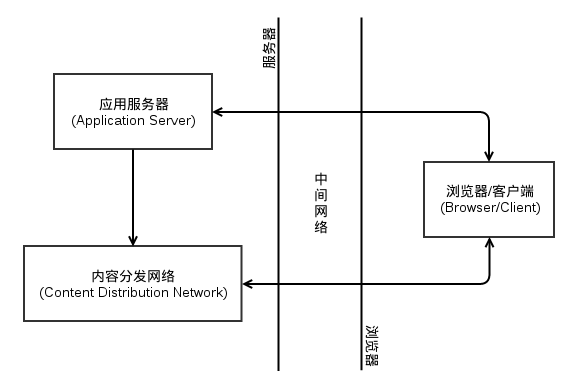
\includegraphics[scale=0.5]{figures/diagram-architecture.png}
    \caption{系统架构示意图\label{Architecture}}
  \end{center}
\end{figure}

基于经典的 Client/Server (C/S) 架构模式。在 C/S 模式的基础上,基于浏览器这一特殊的执行环境(Execution Context),客户端程序并不直接部署在用户终端上,架构中加入了内容分发网络用于分发静态的客户端程序数据。

接下来,与现在典型的 MVVM 应用方式不同\footnote{Angular.js、Knockout.js等流行的JavaScript实现将MVVM作为客户端框架进行实现},我们在C/S的基础架构上,应用MVVM架构(图~\ref{ArchitectureMVVM})

\begin{figure}[!h]
  \begin{center}
    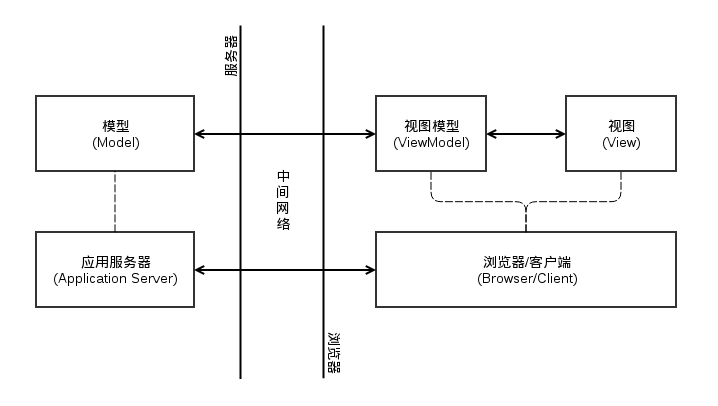
\includegraphics[scale=0.5]{figures/diagram-architecture-mvvm.png}
    \caption{MVVM 系统架构示意图\label{ArchitectureMVVM}}
  \end{center}
\end{figure}

服务器提供MVVM框架中模型(Model)的支持,负责响应业务请求和维护业务数据,客户端提供视图(View)以及视图模型(ViewModel)负责业务数据的呈现逻辑和用户事件的处理\footnote{服务器与客户端之间的通信属于ViewModel的一部分}。

下面将分两个小节分别介绍服务器和客户端的二级架构方案。

\subsection{服务器架构方案}

将服务器部分作为Model进行设计的一大特点是服务器设计的轻量化,这与常见的RIA应用中的服务器设计是基本相符的,服务器为业务数据共享、权限管理等基本需求提供了支持。

\begin{figure}[!h]
  \begin{center}
    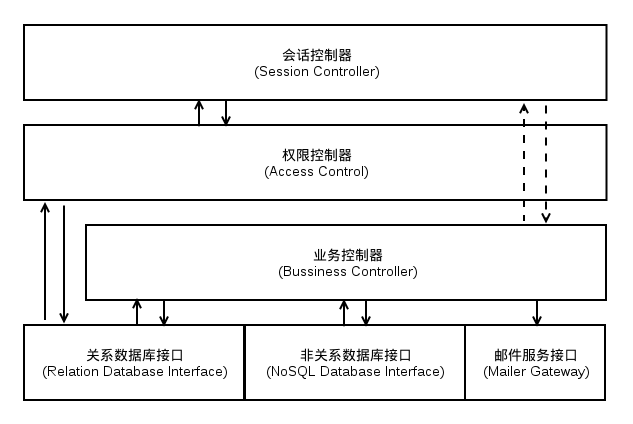
\includegraphics[scale=0.5]{figures/diagram-architecture-server.png}
    \caption{服务器架构示意图\label{ArchitectureServer}}
  \end{center}
\end{figure}

图~\ref{ArchitectureServer} 说明服务器的分层架构模式:

\begin{itemize}
  \item 顶层通过 HTTP/HTTPS 提供的会话层对会话状态进行管理
  \item 权限控制器提供账户服务
  \begin{itemize}
    \item 处理账户登录、注册等账户相关数据业务
    \item 拒绝超出权限范围的访问请求、保障用户逻辑输入的正确性
    \item 向业务逻辑层提供透明的用户认证机制
  \end{itemize}
  \item 业务逻辑层实现产生商业价值的业务逻辑
  \item 最下层为数据持久化以及外部服务层
\end{itemize}

服务器利用混合数据库模式,关系型数据库管理业务数据等强关系关联的数据、非关系型数据库处理会话数据等弱关系数据。(见~\ref{sec:Database})

\subsection{客户端架构方案}

上文中提到客户端实现整体架构中的View以及ViewModel部分

\begin{figure}[!h]
  \begin{center}
    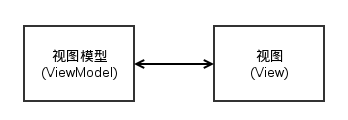
\includegraphics[scale=0.5]{figures/diagram-architecture-client.png}
    \caption{客户端架构示意图\label{ArchitectureClient}}
  \end{center}
\end{figure}

视图 (View) 在系统中被定义为一系列模板的集合,ViewModel 处理页面逻辑,经典 MVVM 模式当中的 DataBinding 模式由特殊的 ViewModel 实现。

\section{数据库设计\label{sec:Database}}

本项目主要使用关系型数据库系统(Relational Database System, RDBS)进行业务数据的管理。

在面向业务的系统构建,特别是 MVVM 模式构建的系统当中,对数据的清晰定义将影响到系统业务的稳定性、可靠性、可扩展性等多个重要的性能。定义良好的数据规格可以直接成为 MVVM 模式中 Model 定义的来源。

本节首先描述课程管理系统数据库的设计概要以及一些需要特别说明的设计概念,后面几个小节描述课程数据、表单数据、用户数据模型的设计方案。

\newpage

\subsection{设计概要}

\begin{figure}[!h]
  \begin{center}
    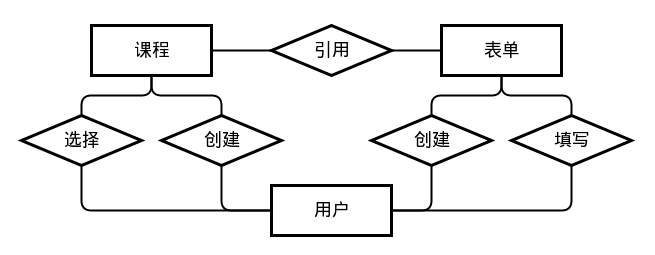
\includegraphics[scale=0.5]{figures/diagram-er-overview.png}
    \caption{数据库E-R关系示意图\label{DatabaseOverview}}
  \end{center}
\end{figure}

系统主要有下面三类业务数据实体:

\begin{itemize}
  \item 课程数据实体
  \item 表单数据实体
  \item 用户数据实体
\end{itemize}

需要特别说明的是 \textbf{表单数据实体} 用于存储系统内其他实体所引用的表单定义。在现实的业务交往过程当中,业务的完成流程往往是基于表格的,创建业务管理系统的核心就在于对表单的创建、维护以及对填写好的表单进行归档、整理。因此,在系统的设计过程中通过创建通用的表单数据实体,将业务数据需求通过表单数据实体进行描述,能避免系统内对业务数据的检索,提高数据库的可扩展性以及系统的业务灵活度。

同时,系统内存在下面业务关系:

\begin{itemize}
  \item 选课业务关联
  \item 表单引用关联
  \item 标签/域关联~\footnote{为了让图形语言表达更清晰,本关联未在图~\ref{DatabaseOverview} 中得到体现。}
  \item 创建者关联
\end{itemize}

\textbf{标签/域关联} 是为了满足系统对系统内数据实体访问权限的细化控制需求而设定的配置数据,这是一组在所有实体上都可以实现的“接口”,实体通过限定“域(Scope)”确定有权限访问该实体的“标签(Tag)”。标签是对“搜索”逻辑的简化和抽象,使用标签机制可以更高效地完成对数据实体的筛选操作,基于标签的检索也能够更有效的保证数据库系统的安全性与可靠性。

\newpage

\subsection{课程实体设计}

\begin{figure}[!h]
  \begin{center}
    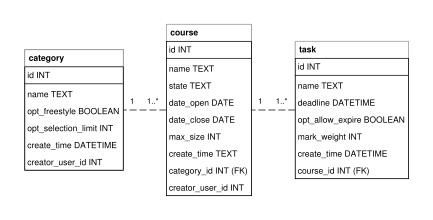
\includegraphics[width=\textwidth]{figures/diagram-eer-course.pdf}
    \caption{课程实体\label{DatabaseEntityCourse}}
  \end{center}
\end{figure}

\textbf{课程(course)} 是与课程管理系统的核心实体,包含了课程的基本信息。

\textbf{任务(task)} 为导师规划课程进展、检测教学成果提供了条件:

\begin{itemize}
  \item 系统可以借助评分权重和每一项任务的评分辅助导师给出学员的课程成绩。

  \item 任务表单由导师维护,添加任务时选取,学生应在截止时间内填写完成表单(作业)并提交,供导师查阅后给出评分。

  \item 任务截止之前(允许超时提交的情况下也包括截止之后)学员可多次提交更新。
\end{itemize}

\textbf{课类(category)} 的设计是为了解决更复杂的选课管理需求:

\begin{itemize}
  \item 课类为每门课程提供一份模板,课类下属的课程需“继承”自该课类(课程类目)
  \item 可由导师定义课类内的选课方案~\footnote{比如,“2010级企业实习实训”课类下,定义每名学员只能选取单一课程,在此课类下创建相关的实习实训职位,自主实习的学生可向负责导师申请添加新的职位信息,导师批准后即给与选取。}
  \item 开放学员选题的课类可由学员向指定导师提交课题,课题信息经过导师审核,经指定导师同意后加入课类
\end{itemize}

\newpage

\subsection{用户/账户实体设计}

\begin{figure}[!h]
  \begin{center}
    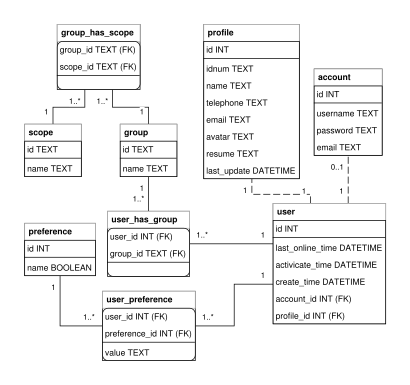
\includegraphics[width=\textwidth]{figures/diagram-eer-user.pdf}
    \caption{用户/账户实体\label{DatabaseEntityUser}}
  \end{center}
\end{figure}

用户在系统内的活动以~\textbf{用户(User)} 实体作为身份标识,\textbf{账户(Account)} 为需要连接的外部身份提供存储支持(如 OpenID 服务)。

数据库配置了基于用户-组-权限的数据结构以存储权限配置,有关权限控制的更多细节请参考~\ref{sec:ServerAPI}。

\newpage

\subsection{表单实体设计}

\begin{figure}[!h]
  \begin{center}
    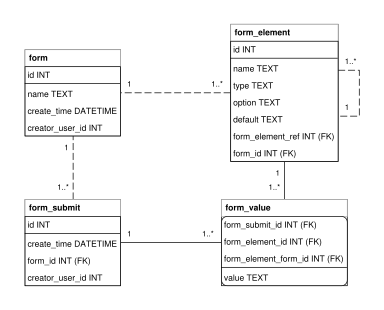
\includegraphics[width=\textwidth]{figures/diagram-eer-form.pdf}
    \caption{表单实体\label{DatabaseEntityForm}}
  \end{center}
\end{figure}

表单项(Form Element) 有如下几种类型~\footnote{表单项类型为类型标识符字符串,由应用逻辑定义并进行解释,数据库仅存储类型标识符与字符串值。}:

\begin{itemize}
  \item 隐藏域(Hidden)
  \item 文本域(Text Input)
  \item 文件域(File)
  \item 图片域(Image)
  \item 地址域(Address/Location)
  \item 单选域(Radio)
  \item 多选域(Checkbox)
  \item 长文本域(Text Area)
  \item 富文本域(Markdown)
  \item 日期域(Date)
  \item 时间域(Time)
  \item 日期/时间(DateTime)
  \item 音频(Audio)
  \item 视频(Video)
  \item 用户(User)
\end{itemize}

值得注意的是 $form\_element$ 定义中包含到 $form\_element$ 的外键用于处理 CheckBox、RadioBox、Selector 等的数据源请求。

\subsection{标签/域模式}

为了解决一系列实体的”搜索“问题(如可见性控制、批量操作),设计标签(Tag)机制给每个可检索实体赋予一组标签。

\begin{figure}[!h]
  \begin{center}
    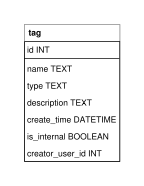
\includegraphics[scale=1.3]{figures/diagram-eer-tag.pdf}
    \caption{标签实体\label{DatabaseEntityTag}}
  \end{center}
\end{figure}

为实体赋予标签需要在实体与标签之间建立多对多的关系,实体的标签能够通过实体的创建者以及管理员进行维护。

实体也能够通过标签进行有效性验证,通过与标签建立多对多的 $filtering$ 关系即可存储有效性验证数据。

\newpage

\section{服务器接口设计\label{sec:ServerAPI}}

服务器接口(通信协议)基于 REST(Representational State Transfer) 服务风格设计~\cite{fielding2002principled}。

\begin{table}[!h]
  \begin{center}
    \noindent
    \ttfamily
    \begin{tabular}{|c|c|l|}
      \hline
      \textbf{符号} & \textbf{资源名} & \textbf{描述} \\ \hline
      u & user      & 用户          \\ \hline
      p & profile   & 用户资料      \\ \hline
      m & message   & 消息          \\ \hline
      g & group     & 课程组(分类)  \\ \hline
      c & course    & 课程          \\ \hline
      t & task      & 任务          \\ \hline
      f & form      & 表单          \\ \hline
      s & submit    & 提交(填表)    \\ \hline
      a & answer    & 答案(任务提交)\\ \hline
      r & review    & 评价(评分)    \\ \hline
      y & registry  & 注册(选课记录)\\ \hline
      e & session   & 会话          \\ \hline
    \end{tabular}
    \caption{URI符号表\label{APURIGlossary}}
  \end{center}
\end{table}

\LTXtable{\linewidth}{parts/table/protocol.tex}

上面的表格给出了服务器开放访问的所有数据资源接口以及接口对访问权限的限制,可以看出通过使用 RESTful 的 API 设计风格,通信协议设计可直接对应参照数据库内的实体设计方法,表~\ref{APURIRelation} 给出的接口之间的关系也对应于数据库实体间的关系。

\begin{table}[!h]
  \begin{center}
    \noindent
    \ttfamily
    \begin{tabular}{|c|l|}
      \hline
      \textbf{符号} & \textbf{资源关系描述} \\ \hline
      (u)/(p) & 用户资料     \\ \hline
      (u)/(m) & 用户消息     \\ \hline
      (u)/(c) & 用户的课程   \\ \hline
      (c)/(m) & 课程消息     \\ \hline
      (c)/(t) & 课程任务     \\ \hline
      (f)/(s) & 表单提交     \\ \hline
      (t)/(a) & 任务答案     \\ \hline
      (a)/(r) & 答案评价     \\ \hline
      (c)/(y) & 课程注册申请 \\ \hline
      (y)/(r) & 课程评价     \\ \hline
      (a)-(s) & 答案引用提交 \\ \hline
      (t)-(f) & 任务引用表单 \\ \hline
      (c)-(g) & 课程引用课类 \\ \hline
      (g)-(f) & 课类引用表单 \\ \hline
    \end{tabular}
    \caption{资源关系表\label{APURIRelation}}
  \end{center}
\end{table}

另外,客户端在访问服务器枚举接口时服务器返回列表内元素的 $id$ 列表,客户端需要对每个元素进行单独访问,这要求客户端有一定的缓存机制作为支持以提升请求性能(或者浏览器支持 HTTP Pipelining 机制)。

\newpage

\section{小结}

本章描述了项目中基于用户需求所进行的系统设计活动:

在系统的体系结构设计当中引入了跨服务器-客户端的 MVVM 模式、确定了轻量服务器的构建模式。

数据库设计遵循关系型数据库设计范式,在保证业务高效和数据一致的前提下为应用层提供了良好的数据可扩展性。

使用 REST 风格制定的服务器接口与数据库设计呈现出高度的一致性。

下一章节将对 ViewModel 与 FRP 做出简单的介绍,导出在对交互实现起到重大作用的 ViewModel 构建方式。


\chapter{MVVM 模式与 Reactive Programming}

本章将用一定的篇幅详细介绍 MVVM 模式在面向对象的过程式编程语言内的设计实现。使用实例解释 Reactive Programming 以及 FRP 的特性,并导出基于 FRP 进行的 ViewModel 实现。

\section{面向对象的 MVVM 实现}

\begin{figure}[!h]
  \begin{center}
    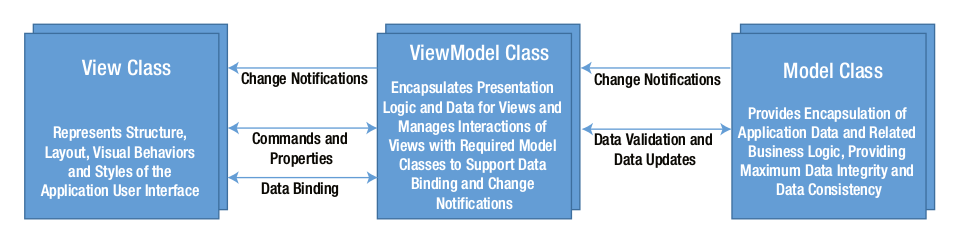
\includegraphics[scale=0.5]{figures/diagram-mvvm-pattern-ref.png}
    \caption{MVVM 设计模式中的关键类~\cite{ghoda2012windows}\label{MVVMCoreClasses}}
  \end{center}
\end{figure}

面向对象的实现中 ViewModel 对象是对观察者模式(Observer Pattern)的一种实现。

\begin{figure}[!h]
  \begin{center}
    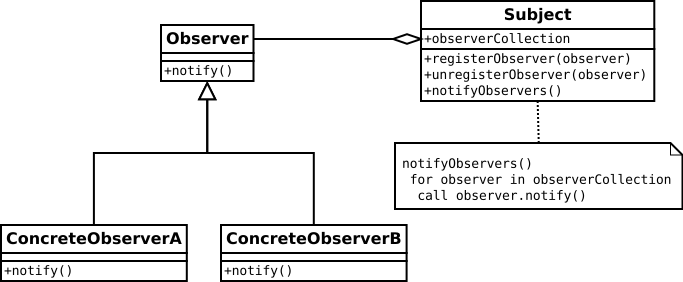
\includegraphics[scale=0.5]{figures/pattern-observer.pdf}
    \caption{观察者模式\label{PatternObserver}}
    Subject 接受注册 Observer 并在 notifyObserver 中向 Observer 推送数据
  \end{center}
\end{figure}

参照类图\footnote{Wikipedia: File:Observer.svg}中的定义对 Model 与 ViewModel 进行定义:

\begin{verbatim}
    @interface IModel implements ISubject;
    @interface IViewModel implements IObserver;
\end{verbatim}

为了让 ViewModel 具有 Model 的特性,将 ViewModel 的接口改写为:

\begin{verbatim}
    @interface IViewModel implements IObserver, IModel;
\end{verbatim}

\begin{figure}[!h]
  \begin{center}
    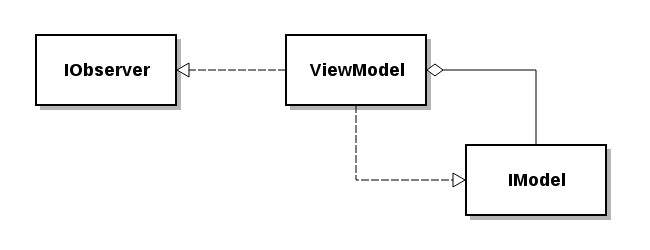
\includegraphics[scale=0.5]{figures/diagram-viewmodel.png}
    \caption{ViewModel 类图\label{ViewModelClass}}
  \end{center}
\end{figure}

ViewModel 通过订阅 Model 获取 Model 的数据变更(图~\ref{MVVMCoreClasses} 中 Model 至 ViewModel 的 $Change Notifications$)。与之类似,View 与 ViewModel 之间的 Binder 定义:

\begin{verbatim}
    @interface IBinder implements ISubject, IObserver;
\end{verbatim}

Binder 实例构造时指定 View 元素作为 Observer 实例,指定 ViewModel 元素作为 Subject 实例就可以建立 ViewModel 至 View 的单向绑定关系。双向绑定关系由两个单项绑定构成,不加赘述。

值得一提的是,由于 ViewModel 同时实现了 Model 接口,具备了 Model 的行为特性,ViewModel 之间也是可以互相观察的:

\begin{figure}[!h]
  \begin{center}
    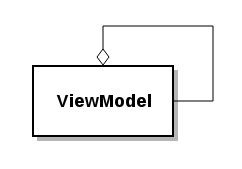
\includegraphics[scale=0.5]{figures/diagram-viewmodel-cascading.png}
    \caption{ViewModel 的可级联特性\label{ViewModelCascading}}
  \end{center}
\end{figure}

这样的设计使得ViewModel模式获得了很强的可扩展性,将用户交互状态分开给不同的 ViewModel 进行管理可以显著减小业务逻辑状态的维护难度,开发者可以利用封装的 ViewModel 类库进行组合来完成用户交互逻辑的实现,具有很高的可复用性。使用 ViewModel 进行开发也同时带来了良好的可测试的代码结构。

通过上面的分析可以看出,观察者模式是 MVVM 模式的重要基础。下一节~\ref{sec:AsyncProgrammingModel} 从编程模型的角度讨论使用观察者模式的合理性并引出FRP作为异步编程模型的解决方案。

\section{用户交互与异步编程模型\label{sec:AsyncProgrammingModel}}

用户与计算机的交互是基于人机交互界面(UI)进行的,早期的终端用户界面 (Console User Interface, CUI) 程序与用户进行同步交互,交互的模型为: 用户输入-程序执行-程序输出-用户输入\ldots,这样的逻辑在面向过程编程的语言实现中是非常自然的程序表达——按先后顺序执行每一条语句。

在图形界面(Graphical User Interface, GUI)得到应用之后,用户可以不间断地与程序进行交互而不需要等待程序的执行,这样的设计极大的提升了用户体验。现代的 GUI 程序广泛使用了事件模型处理用户交互,事件是一组时间顺序的离散数据的集合,对程序来说事件是一类异步产生的数据,因此,基于事件进行编程便成为了进行用户交互实现的基本方法。

明确了这点之后,我们可以将行用户交互实现的本质问题归结为~\textbf{处理异步事件}。

基于事件的开发并不是命令式(Imperative)编程模式所擅长的领域,也导致了大多数 GUI 程序的交互实现都极其不易维护。

以 Drag'n'Drop (拖放操作, DnD) 为例\cite{Zhao2010},在 GUI 上实现 DnD 操作需要程序监听三个不同的 GUI 事件:

\begin{itemize}
  \item 在 MouseDown 事件中标记 isDragging (正在拖动)
  \item 在 MouseMove 事件中判断 isDragging 并且开始绘制拖放光标、使用 API 获取拖放的数据
  \item 在 MouseUp 事件中判断 isDragging 并结束拖放状态(停止绘图)
\end{itemize}

在命令式编程语言中往往使用回调函数(Callback Function)对事件进行处理,这种离散的逻辑碎片导致了在 GUI 实现中出现大量的碎片代码以及全局状态,破坏了“代码逻辑局部性”、“变量局部性”等有利于代码组织和维护的性质。

鉴于这种直接使用回调函数编程的弊端,面向对象的命令式编程语言使用观察者模式(Observer Pattern),利用观察者响应事件数据从而实现对代码的封装管理。

\begin{verbatim}

    @class DnDObserver implements IObserver
      private boolean isDragging;
      private Coord   prevCursorPosition;
      public void notify(propName, oldValue, newValue);

    @interface ObservableView implements ISubject

\end{verbatim}

$ObservableView$ 将事件抽象为一系列数据以及对属性变更事件的触发,$DnDObserver$ 监听 $ObservableView$ 的属性变更,这样的实现维护方便、有较强的可复用性。

异步事件的处理逻辑符合声明式(Declaritive)语言自然的表达方式,使用声明式语言进行用户交互实现的尝试也越来越多。下一节将介绍的的 FRP 方法在异步事件处理方面就有非常出色的性能。

\section{Reactive Programming 与 Monad 函数}

Reactive Programming 的概念继承自 FRP,随着越来越多的语言融入和函数式语言的开发方法,Reactive 模式也被越来越多的应用在 GUI 应用的开发中~\footnote{http://www.reactivemanifesto.org/}。

以 Reactive.js~\footnote{此处使用的是 Reactive.js 的最小 Reactive 核心} 为例~\cite{Carkci2013}

\begin{verbatim}

    // Declaration
    var A = $R(function (b, c) { return b + c });
    var B = $R.state(2); // Initial value for B
    var C = $R.state(1); // Initial value for C
    A.bindTo(B, C); // Declare B and C as argument for A

\end{verbatim}

上面的代码片段演示了 $A = B + C$ 的 Reactive 定义(使用 JavaScript 语言环境),当更改 $B$ 或 $C$ 的值发生改变时 $A$ 的值便会“自动”重新计算。

\begin{verbatim}

    // Reaction
    A();   // -> 3
    B(5);  // Set B to 5
    A();   // -> 6

\end{verbatim}

Reactive 定义中出现的 $\$R$ 函数所产生的对象(即 A、B和C)在纯函数式编程语言中被命名为 Monad~\cite{raey}。

FRP 的将系统抽象为 $行为(Behaviors)$ 和 $事件(Events)$,上例中先使用 Monad 函数包装行为(见 A、B、C 的定义)并在行为之间建立关联(上例中使用 $bindTo$),然后通过传入事件($B(5);$) 更改“行为”的值。

不难发现,Monad 与 Observer 模式有非常相似的行为方式,而且对于具有丰富函数式开发能力的 JavaScript 来说 Monad 能带来更清晰简洁的过程描述。

\section{小结}

本章讨论分析了面向对象 MVVM 模式实现的基础模式——Observer 模式,并举例说明了 Observer 模式在处理异步事件方面较传统的过程式实现方法所具有的优势。

本章还通过实例分析了 Reactive Programming 中 Monad 的应用,详细说明了 Monad 的行为以及与 Observer 的相似性,本项目实现 MVVM 架构的过程中将应用 Monad 结构对 ViewModel 进行开发。


\chapter{实现}

本章整理总结系统实现过程中遇到的关键问题的解决方案以及解决问题的过程中进行的探索性过程。\footnote{考虑到表述紧凑性,本章节仅包含描述解决方案所必须的代码片段,详细的代码实现请参考附录内的相关内容}

\section{开发环境与技术选择}

图~\ref{TechStack} 所示为最终确定的系统实现环境和进行的技术选择: 系统开发主要使用 JavaScript 语言平台,应用服务器端使用 Node.js 而客户端使用 JavaScript 脚本开发业务代码。

\begin{figure}[!h]
  \begin{center}
    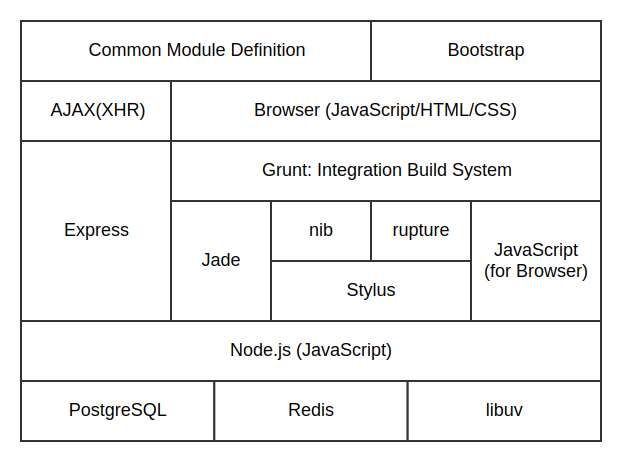
\includegraphics[width=\textwidth]{figures/techstack.pdf}
    \caption{系统开发环境与组件\label{TechStack}}
  \end{center}
\end{figure}

相较 Java/.NET 等流行的企业级解决框架,Node.js 支持函数式编程范式,在 Express 框架的帮助下可以快速的搭建稳定的服务器应用。另外,选择 Node.js 的一大原因是 Node.js 采用消息队列机制,并支持异步 I/O 操作,单线程异步操作模型可以有效的减少内存开销,同时,避免了传统服务器开发过程中所容易出现的线程同步问题,极大的提升了服务器的稳定性。对轻量服务器设计来说使用 Node.js 能够在取得良好的服务器性能以及稳定性的同时达到最大的开发效率。

客户端代码使用 Grunt 集成编译系统进行独立编译,相比使用 Express 进行线上编译-缓存的策略,使用 Grunt 集成编译环境直接将客户端程序编译为线上版本有利于前端服务器直接对文件进行缓存操作,将客户端资源编译工作从应用服务器中分离出来也有利于应用服务器自身的可扩展性和运行时性能。

\section{服务器(Model)}

应用服务器的职能在系统中主要负责多用户会话维护、权限控制以及数据操作。

\subsection{轻量级 Object-Relation Mapping 实现}

Object-Relation Mapping (ORM) 是将数据库关系与数据库实体的数据直接通过面向对象封装进行访问的一种方法。

服务器对数据库的业务访问逻辑普遍包含:

\begin{itemize}
  \item 验证业务数据有效性
  \item 转换业务数据(如 进行 Password Hash)
\end{itemize}

为了提高数据库访问代码的复用程度,项目中设计了 $querybuilder$ 轻量级数据库 ORM 框架,以用户资料管理为例:

\begin{verbatim}

        profile: {

          update: qb('INSERT INTO profile SET ? ON DUPLICATE KEY UPDATE ?', {
            user_id : Number,
            name    : String,
            gender  : String
          }),

          query: qb([
            'SELECT a.`user_id` AS `user_id`,',
            '       p.`name`    AS `name`, ',
            '       p.`gender`  AS `gender`,',
            'FROM `account` a INNER JOIN `profile` p ON a.user_id = p.user_id',
            'WHERE a.`account` = :account AND a.`domain` = :domain'
          ].join(' '), { account: String, domain: String })

        },

\end{verbatim}

$qb$ 函数返回用于数据库查询的高阶函数,在中间件中:

\begin{verbatim}

        db.profile.update(req.data, function (err, result) {

          if (err) {
            return next(new ApplicationError({
              message: 'Failed to update user profile',
              cause: err
            }));
          }

          return res.status(200).end();

        });

\end{verbatim}

通过使用简单的 ORM 框架,对 SQL 语句模板进行集中统一的管理,让业务逻辑代码得到了高效的组织。

\subsection{权限控制中间件}

中间件是 Express.js 服务器框架所使用的基本设计模式。

\begin{figure}[!h]
  \begin{center}
    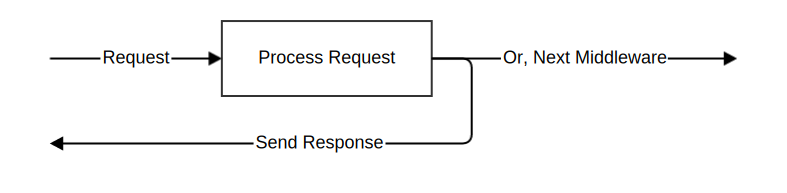
\includegraphics[width=\textwidth]{figures/pattern-middleware.pdf}
    \caption{中间件模式典型交互示意图\label{ExpressMiddleware}}
  \end{center}
\end{figure}

如图~\ref{ExpressMiddleware},中间件获得请求以后 Express.js 会按照中间件的注册顺序使用中间件处理请求,中间件返回三种处理结果:

\begin{enumerate}
  \item 处理完成,发送响应数据
  \item 进行数据变换,发送至下一个中间件
  \item 处理失败,使用错误处理中间件进行处理
\end{enumerate}

权限控制中间件用于实现服务器接口的权限控制(见~\ref{sec:ServerAPI})。

权限控制中间件通过传入的高阶函数判断当前对接口进行的请求的合法性:

\begin{verbatim}

        app.post('/c/:id/t/',
          // role of current user is admin or teacher
          accessctl(role('admin'), role('teacher')),
          // can access c of :id with current request
          accessctl(from('/c/:id/', 'c')),
          function (req, res, next) {
            // Bussiness code
          }
        )

\end{verbatim}

上面的例子中 $role$ 与 $from$ 分别是用于确认用户角色以及其他接口访问能力的~\textbf{权限策略},$accessctl$ 通过执行权限策略并检查策略的执行结果决定是否给予当前的请求进行下一步中间件。

除了应用于对某个接口的权限控制,$accessctl$ 还可以通过 $express.use$ 方法配置一组 $router$ 的权限。

\section{客户端视图模型(ViewModel)}

项目中使用 Monad 对 MVVM 模式中 ViewModel 进行实现,替代面向对象设计中的 Observer 模式。Monad 与 Observer 都能合理的组织代码,将代码复杂度保持在线性增长的状态,而 Monad 在函数式开发环境中更容易实现和使用。

本项目尝试开发的 Entangle 框架经过三次迭代最终满足客户端前端开发的需求,Entangle 框架使用 Monad 作为 Reactive Programming 的响应核心,并在此基础上封装 Builder 模式以简化对业务逻辑中经常出现的顺序逻辑的定义过程。下面几个小节对 Entangle 框架成型过程中所解决的重要业务需求以及其实现方案进行叙述。

\subsection{数据同步}

与服务器进行数据交互是客户端的基础功能之一。

通过 $http$ 转换子(Converter)实现从服务器拉取数据:

\begin{verbatim}

        entangle().http('GET', '/u').pick(function (data) { /* ... */ });

\end{verbatim}

Entangle 使用链式表达式构建串行关系的转换子(Converter),上例实现获取用户信息的功能。

对于轮询的情况,可以使用 $timeout$ 转换子:

\begin{verbatim}

        var juice = entangle().http('GET', '/u')
        var timer = entangle().timeout(2000);

        timer.fork(juice);
        juice.fork(timer);

\end{verbatim}

$fork$ 原语将 timer 的值转发到 juice,当 timer 触发时,触发事件会传递给 juice、发出 http 请求,请求完成后 juice 又会将数据 fork 回 timer 进行下一个 $2s$ 的等待。这样就造成了一个轮询的数据流。

详细的实现请参考附录内容,在这里我们不详细展开 Entangle 的实现细节。

\subsection{页面导航}

页面导航栏的逻辑是单一对象数据绑定的比较典型的实现。entangle 通过自动改写的 jQuery 方法实现对用户界面元素的操作,下面这些代码来自 pilot.js:

\begin{verbatim}

        entangle()
        .location()
        .pick().string('.navbar-collapse a[href="{{pathname}}"]')
        .$().$parent('li').$addClass('active')

\end{verbatim}

$string$ 转换子将输入的数据代入字符串模板,$\$$ 转换子将输入的字符串转换为 jQuery 对象之后以 \$ 开始的转换子都经过自动改写指向对应的 jQuery 方法。

$location$ 转换子实现对页面地址信息的监听:

\begin{verbatim}

        location: function () {

          var converter = function () {
            this.resolve(location);
          };

          // get location from window object
          var location = {
            host: window.location.host,
            hostname: window.location.hostname,
            protocol: window.location.protocol,
            search: window.location.search,
            href: window.location.href,
            port: window.location.port,
            pathname: window.location.pathname,
            hash: window.location.hash,
          };

          // listen for hash change event
          $(window).on('hashchange', function () {
            location.hash = window.location.hash;
            converter.resolve(location);
          });

          return converter;

        }

\end{verbatim}

这里介绍一下转换子的构成:

\begin{itemize}
  \item 转换子是一个返回高阶函数的函数
  \item 转换子内可以定义自己的闭包状态
  \item 转换子可以进行事件监听
  \item 转换子使用 $resolve$ 方法将数据传输给后继转换子
\end{itemize}

另外,这里需要特别说明的问题是,基础的转换子实现是基于面向过程的编程方法的,事实上 Haskell 在描述具体的“怎么做”(HOW)逻辑的时候也使用 $do$ 语法糖模拟顺序执行的代码(通过参照代码行之间的前后依赖关系,在定义“是什么”(WHAT)的情况下依赖关系是由“是什么”定义的,不参照代码行的前后依赖关系),这也是支持混合语言特性的语言的优势所在。

\subsection{绑定列表数据}

第三版的 entangle 对列表数据的绑定做出了设计,第二版 entangle 中使用 entangle 核心对上下文进行切换管理,这样做所产生的代价是核心代码的大量冗余与不可扩展性,因此,第三个版本的 entangle 采用了 monad 的封装机制,仅实现最核心的 Reactive 需求。在做出了这样的修正之后,编写清晰的列表数据的绑定逻辑成为可能。

\begin{verbatim}

        init: entangle().json('get', '/c/').pick('data')

\end{verbatim}

首先,$init$ 从服务器获取对象 id 列表,然后 id 列表数据被传送到 $list$ 进行扩展:

\begin{verbatim}

        list: entangle().collect(_.identity).each(function () {
          // return [Entangle Object]
        })

\end{verbatim}

为了处理列表数据条目的增加与删除,我们需要从列表项中提取出没个项目的唯一 id,并构造字典,这一工作由 $collect$ 转换子完成。

接下来将整个列表传入 $each$ 转换子,$each$ 转换子接受一个产生转换子的函数作为参数(factory 函数),$each$ 转换子内部会为不同的元素分别调用 factory 函数产生对应的转换子,由产生的转换子管理子元素的状态。

特别地,转换子内需要判断转换子所管理的元素是否已经被删除。

\subsection{数据缓存与按需触发}

性能因素是 FRP 的缺点之一~\cite{Elliott:2009:PFR:1596638.1596643},对计算结果做缓存以及按需触发控制能够有效的减小性能开销。

entangle 设计了 $sponge$ 用于缓存输入的数据结果与控制触发信号的输出。

\begin{verbatim}

        entangle()
        .string('/u/0/p').json('get').pick('data')
        .sponge()
        .$('.view-photo-img').$attr('src', '{{photo}}')

\end{verbatim}

此处设置了 $sponge$ 转换子,则在用户资料没有发生改变的情况下不通知 $\$('.view-photo-img')$ 对象改变其 src 属性

$sponge$ 转换子提供 $alwaysTrigger$ 参数来配置触发行为,若使用 $sponge(true)$ 则后继转换子不论 sponge 内的缓存是否更新都会得到触发信号。

\subsection{代码调试工具和策略}

在设计 entangle 的 API 的过程中进行了许多的调试工作,在异步编程的环境下进行调试无法像在同步环境内进行单步跟踪那样对异步代码进行切实的跟踪。异步代码的“单步”调试的实现要依靠调试人员在调试时人工进行动态的断点调整来实现,这也是极其麻烦的一项工作。

为了使用户能够方便的调试 entangle 数据流,entangle.debug 函数集包含了 entangle.logger 和 entangle.breakpoint 转换子,这些转换子不会影响业务数据的传递,entangle.logger 会在 console 输出到达的数据而在程序执行到 entangle.breakpoint 时会提示调试器进行中断,以方便调试人员找到异步事件的调试入口。

虽然这些调试机制还不是相当完善,在一定程度上辅助以适当的调试策略还是能够取得非常良好的调试效果。

\section{客户端视图(View)}

View 的开发使用了 Jade(HTML预处理器) 和 Stylus (CSS预处理器) 组合。使用预处理器进行视图开发有下面几个优势:

\begin{itemize}
  \item 代码冗余度低
  \item 视图元素/样式复用
  \item 模块化视图开发
  \item 可实现简单视图逻辑
\end{itemize}

\begin{figure}[!h]
  \begin{center}
    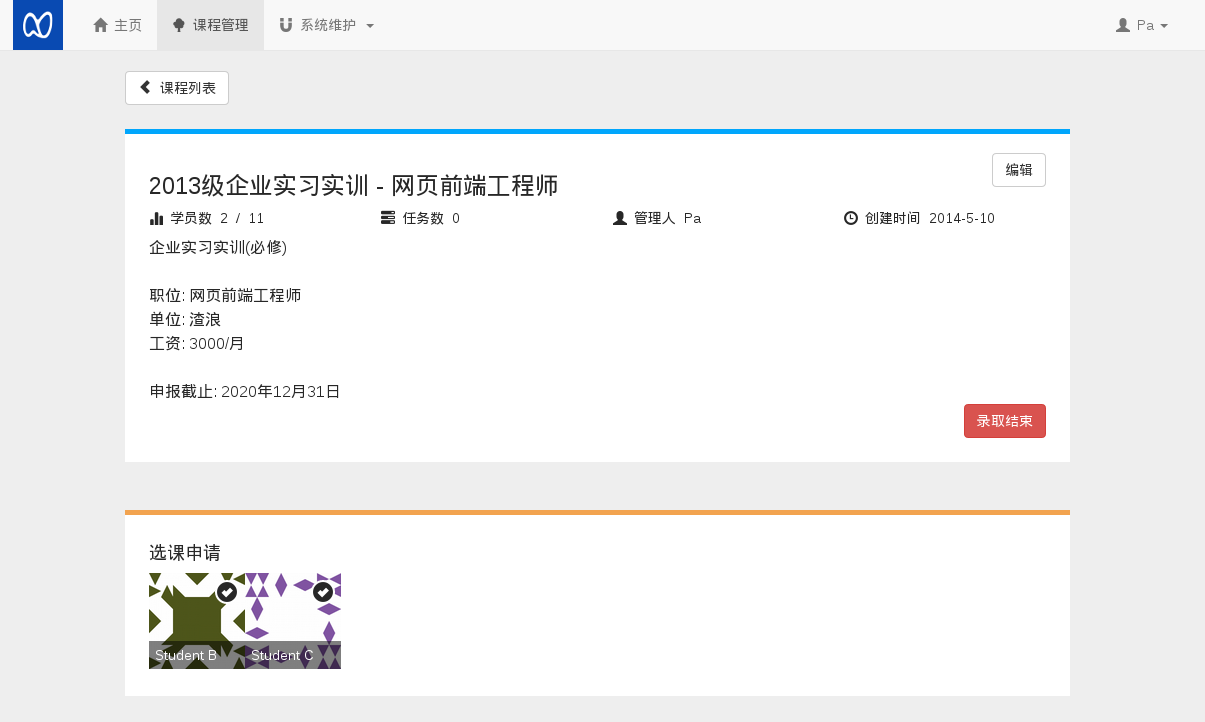
\includegraphics[scale=0.3]{figures/screenshot/enroll.png}
    \caption{视图: 学员录取\label{SSEnroll}}
  \end{center}
\end{figure}

\begin{figure}[!h]
  \begin{center}
    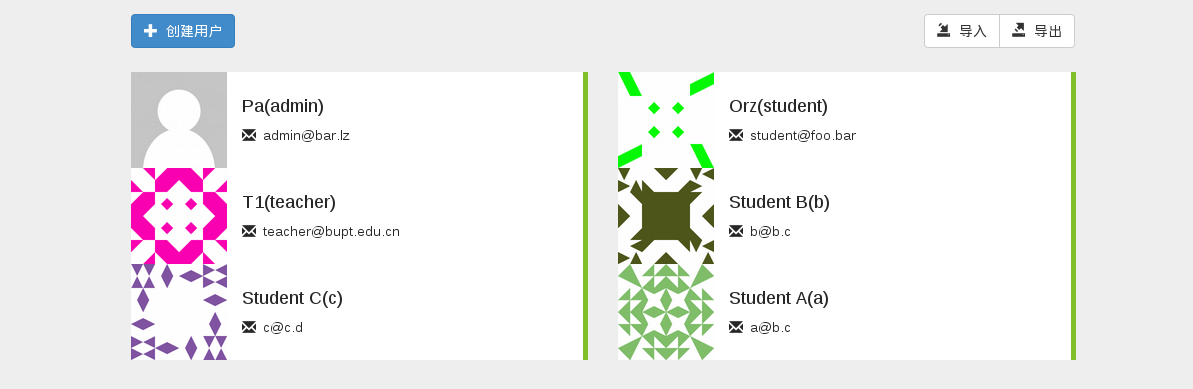
\includegraphics[scale=0.3]{figures/screenshot/userman.png}
    \caption{视图: 用户管理\label{SSUserMgr}}
  \end{center}
\end{figure}

\begin{figure}[!h]
  \begin{center}
    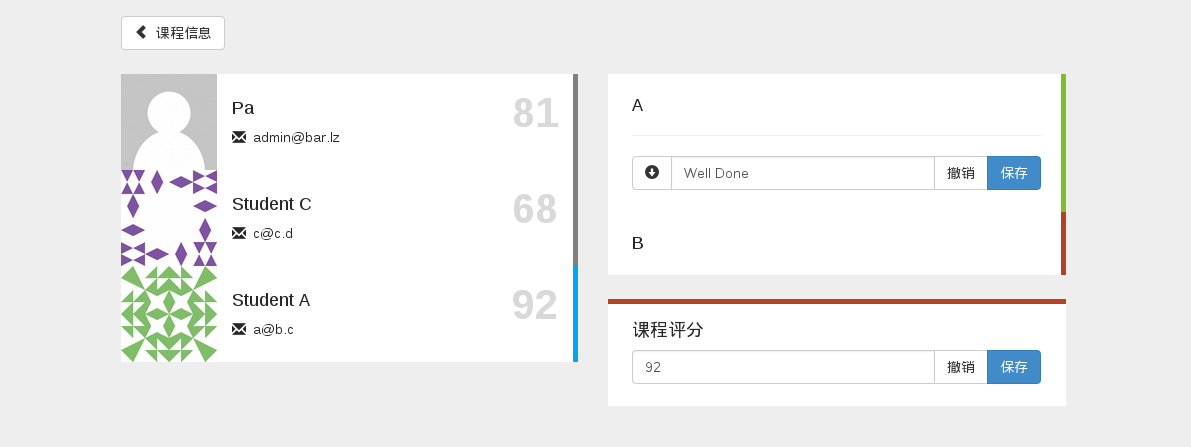
\includegraphics[scale=0.3]{figures/screenshot/review.png}
    \caption{视图: 课程评分\label{SSCourseReview}}
  \end{center}
\end{figure}

\begin{figure}[!h]
  \begin{center}
    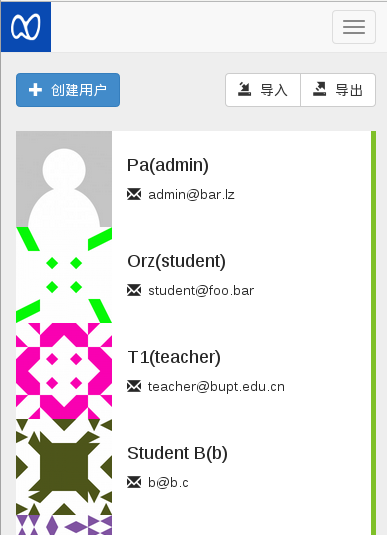
\includegraphics[scale=0.5]{figures/screenshot/responsive.png}
    \caption{视图: 用户管理(移动终端)\label{SSResponsive}}
  \end{center}
\end{figure}


\chapter{总结与展望}

关于系统设计及实现至此就全部阐述完成了,在系统设计过程中遇到许多设计困难,在设计方面做了许多尝试、走了不少弯路。本章对整个毕业设计的过程、毕业设计的过程中所出现的各种问题做一个总结。另外,本章还对将来的一些研究做出一些展望。

产品设计的过程其实就是建模的过程,对产品业务的设计归纳为数据库模型,而用户交互设计则归纳为交互模型,在产品设计的过程当中

\section{MVVM~架构与~Reactive~UI}

由于接触过 WPF 框架下的 MVVM 模式,在开始毕业设计之初的目的就是在 JavaScript 的平台上实现一个 MVVM 框架并进行一次正式的 MVVM 开发实践,随着研究的深入,我对 MVVM 架构的理解也变得更加透彻起来,也认识到 Observer 模式在解决异步编程方面发挥着的重要作用。我个人对于小而美的架构设计有强烈的偏好,所以开始尝试设计一款轻量级的 MVVM 架构应用到项目中。

在函数式语言的领域内我找到了一个答案—— Functional Reactive Programming。后来在研究过程中我发现 Observer 与 Monad 的共同点,而 Monad 所采用的模式能够被 JavaScript 轻易地实现,于是就产生了 Model-View-ReactiveModel 模型(使用 Monad 替代 Observer 的 MVVM 实现)。

在项目中的这个实现命名取自量子纠缠(Entanglement),作为尝试性的实现,Entangle 虽然能够达到维护客户端数据的目的,但也还是存在着一些不足。

虽然已经将 entangle 的核心设计减小到了一定的程度,entangle 在 API 的定义上还没有经过梳理,易用性和代码可读性上都不能真正达到产品的标准~\cite{Gerken:2010:UCM:1753846.1754082}。这些不足体现在:

\begin{itemize}
  \item 建立 Monad 之间关系的过程较繁杂
  \item 与外部库对接上存在 API 接口一致性问题
  \item 受到 Builder 模式的限制,不同类型的转换子无法分类管理
  \item 内存管理模型不明确,存在一定风险
\end{itemize}

出于 API 的简洁性和易用性考虑,我将 entangle 设计为 Builder 模式的结构,Builder 模式隐藏了 Monad 之间关系建立的细节,但是随着项目的开发,Builder 模式的局限性也逐渐显示出来。首先,在 Builder 模式中无法实现对转换子命名空间,也就失去了对转换子进行分类管理的能力; 其次,Builder 模式受制于 JavaScript 语言平台在 API 接口上存在不公平,比如使用“点”操作定义串接 (flow) 关系而使用 $fork$ 函数定义并联关系; 另外,当前实现的 entangle 的语义并不完全,应对某些复杂的关系时难以使用(比如循环逻辑)。

JavaScript 拥有非常丰富的第三方库支持,对 DOM (Document Object Model) 的操作也离不开 jQuery 库的支持,现在的 entangle 仅能够通过 monkey patch 的方法将部分 jQuery 方法自动转换为 entangle 构造器方法,诸如事件注册类的 jQuery 方法只能通过编码实现,对函数式编程扩展库 underscore 和 lodash 也是相同的状况。

\section{研究展望}

接下来的开发工作希望在课程管理系统的实践基础上,将业务逻辑从课程管理延伸到通用 OA 应用领域、实现更灵活的控制配置。这些工作需要更复杂的需求和数据库结构进行支撑。

架构研究方面,为了克服上文提到的一些不足,考虑在 JavaScript 的基础上设计或选择一门编译至 JavaScript 代码并且能够与 JavaScript 执行环境进行互操作的函数式语言用于定义 ReactiveModel 以解决 JavaScript 语言平台的局限~\cite{Freeman:2012:HLW:2480361.2371413},使用更简单的形式定义 Monad 之间的关系。另一方面,接下来还将计划对内存控制模型进行分析和定义,增加内存保护措施,提高程序可靠性。

未来的研究还将更进一步探索 Monad 在图形界面开发之外的应用,尝试将 Reactive Programming 应用在面向事件的服务器平台开发中。



%参考文献
\clearpage
\phantomsection
\addcontentsline{toc}{chapter}{参考文献}
{
  \songti\zihao{5}
  \bibliographystyle{IEEEtran}
  \bibliography{IEEEabrv,reference}
}

%致谢
\clearpage
\phantomsection
\addcontentsline{toc}{chapter}{致\quad{}\quad{}谢}
%\chapter*{致\qquad 谢}
\songti\zihao{-4} 

	本毕设的完成得到了很多人的帮助。首先要感谢清华大学医学院神经工程实验室的洪波老师给了我这次机会在他指导下完成毕设。实验室的高小榕老师在毕设期间也给与了我很多的指导,子钟同步的方案就是在他的提议才完成的。最后还要感谢神经工程实验室的Director高上凯教授,清华大学医学院的王广志教授以及本人本科所在学校北京邮电大学,我能跨校跨专业顺利完成本毕设的任务,离不开学校政策和上级老师的支持。

	此外,在本毕设的完成过程中,我还得到了清华大学医学院神经工程实验室很多学长和学姐的帮助。感谢胥红来学长在我整个毕设过程中对于技术方面和思考问题方式方面的指导和帮助;感谢张丹学长从一开始就给予我的热情支持和鼓励;感谢高海洋师兄对我论文格式排版等方面的指点;感谢钱天翼学长在Matlab处理数据上的指导以及在最后毕设答辩PPT中提出的建议;感谢肖小军工程师帮我完成了QFN封装芯片的焊接以及其他技术方面的支持;感谢宾广宇学长,黄肖山学长还有刘涛学长在计算机端数据处理程序方面的支持,另外刘涛学长提供给我的一些文献帮助我很快入门。感谢郭靖学姐在文献阅读方面的指导,她慷慨的提供了硕士论文原稿给我做为参考;

	本毕设所完成的无线同步触发器协议设计与实现中还有不少问题,由于时间的原因并没有给与完善,衷心希望我所做的工作能为未来该系统的完善提供一些方便。




%附录
\clearpage
\phantomsection
\addcontentsline{toc}{chapter}{附\quad{}\quad{}录}
\chapter*{附\qquad 录}

%XXX 附录图索引
\setcounter{figure}{0}
\renewcommand{\thefigure}{A-\arabic{figure}}

%XXX 附录图索引
\setcounter{table}{0}
\renewcommand{\thetable}{A-\arabic{table}}

\section*{附录~1\quad	课程管理系统业务过程模型}
\label{sec:appendix-bpm}

本节为图~\ref{BPMOverview} 提供展开补充。

\begin{figure}[!hbp]
  \begin{center}
    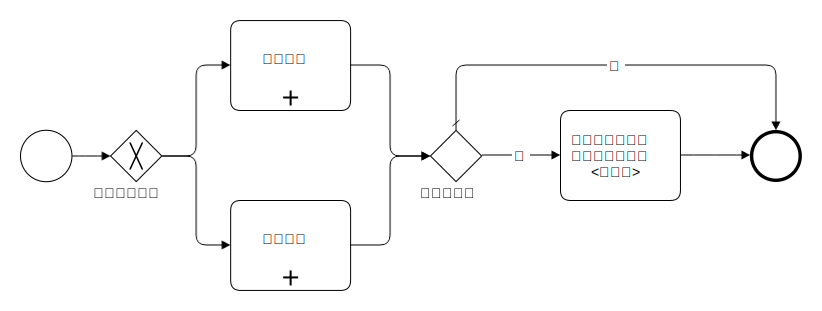
\includegraphics[width=\textwidth]{figures/bpm-cs.pdf}
    \caption{业务过程模型示意图(选课)\label{BPMCourseRegister}}
  \end{center}
\end{figure}

\begin{figure}[!hbp]
  \begin{center}
    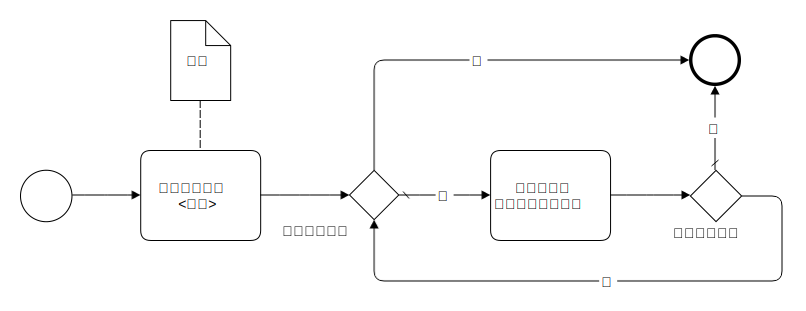
\includegraphics[width=\textwidth]{figures/bpm-cs-pref.pdf}
    \caption{业务过程模型示意图(选课-志愿)\label{BPMCourseRegisterP}}
  \end{center}
\end{figure}

\begin{figure}[!hbp]
  \begin{center}
    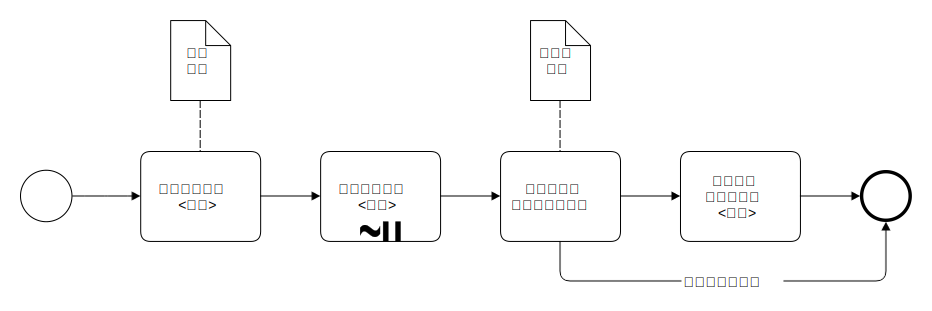
\includegraphics[width=\textwidth]{figures/bpm-cs-dual.pdf}
    \caption{业务过程模型示意图(选课-双选)\label{BPMCourseRegisterD}}
  \end{center}
\end{figure}

\begin{figure}[!hbp]
  \begin{center}
    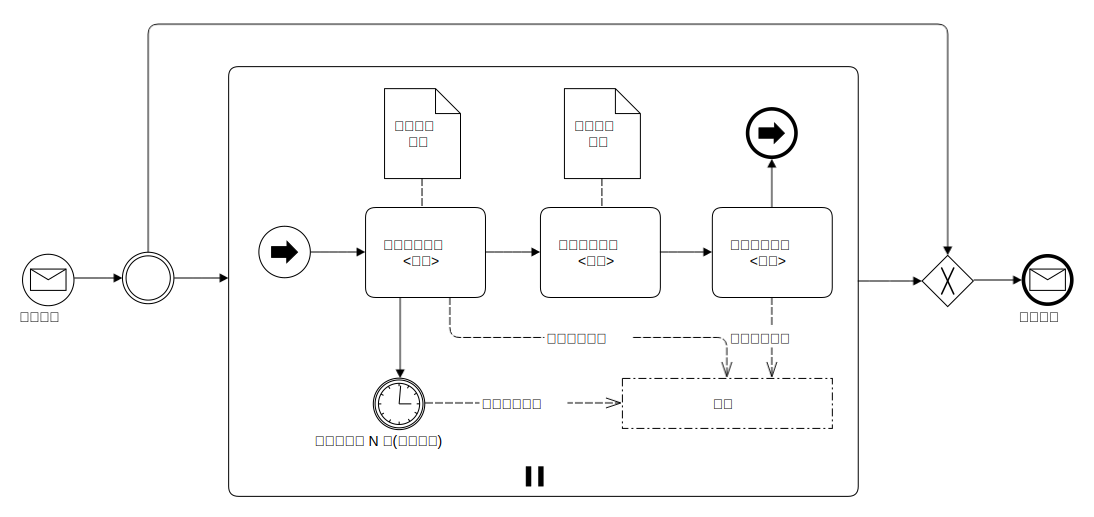
\includegraphics[width=\textwidth]{figures/bpm-task.pdf}
    \caption{业务过程模型示意图(课程任务)\label{BPMTask}}
  \end{center}
\end{figure}

\newpage

\section*{附录~2\quad	课程管理系统产品需求表格}
\label{sec:appendix-requirement-table}

\LTXtable{\linewidth}{parts/table/requirement.tex}

\newpage

\section*{附录~3\quad	数据库设计示意图}
\label{sec:appendix-database-diagram}

图~\ref{FullDatabaseDesign} 展示了完整的数据库设计视图:

\begin{figure}[!h]
  \begin{center}
    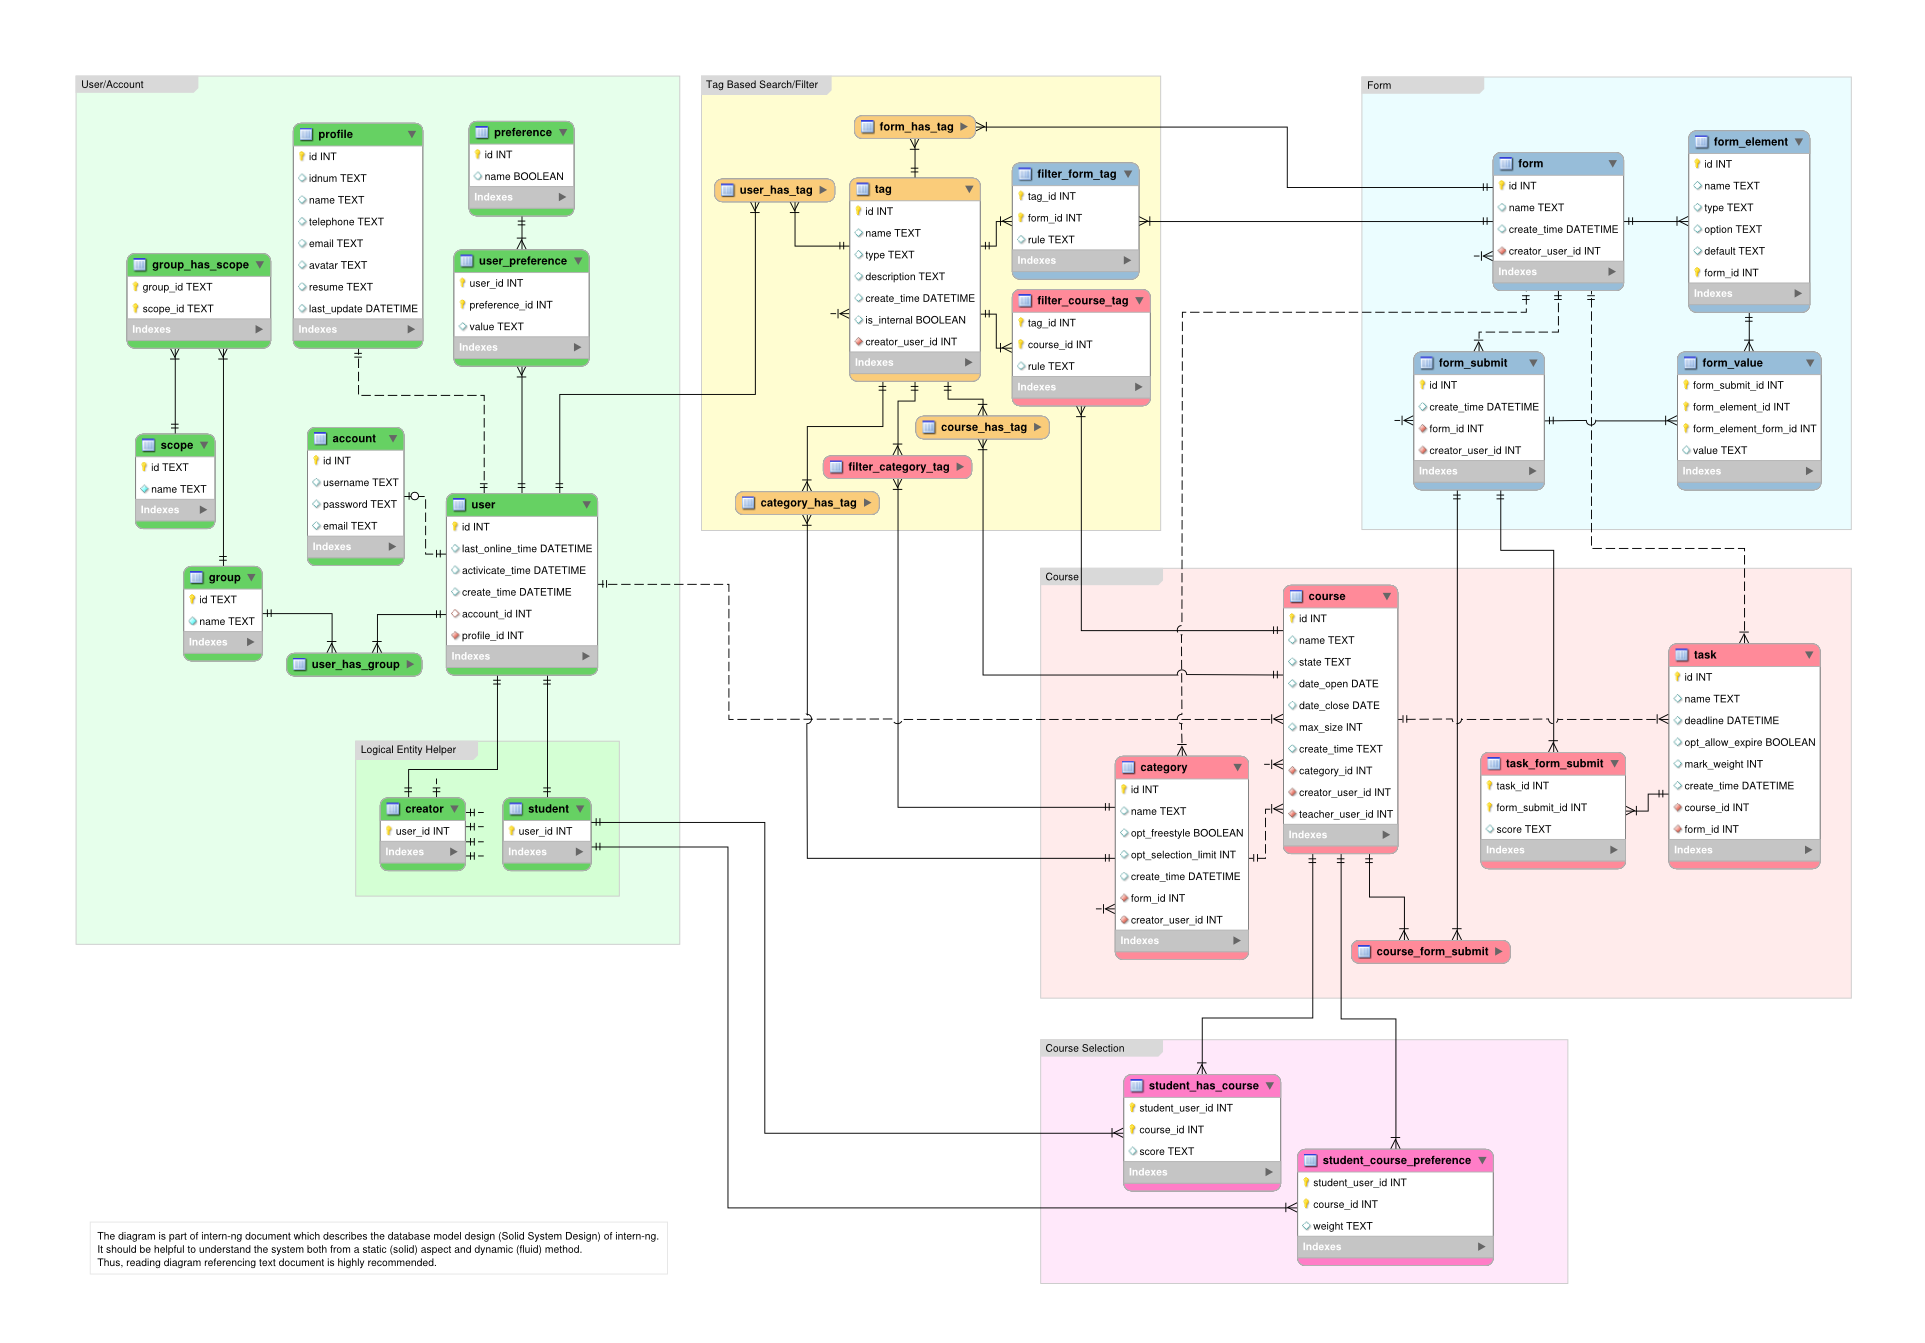
\includegraphics[angle=90, scale=0.5]{figures/eer-120dpi.png}
    \caption{数据库设计视图\label{FullDatabaseDesign}}
  \end{center}
\end{figure}

\newpage

\section*{附录~4\quad	QueryBuilder 模块实现}

\verbatiminput{parts/code/querybuilder.js}

\newpage

\section*{附录~5\quad	Entangle 核心实现}

\verbatiminput{parts/code/entangle.js}



\pagestyle{empty}
%外文资料(译文/原文)
\addcontentsline{toc}{chapter}{外\quad 文\quad 译\quad 文}
\chapter*{外\quad 文\quad 译\quad 文}
\pagestyle{empty}

\begin{center}
{\heiti\zihao{3}Brain Computer Interface System: Progress and Prospects

\textsl{By Brendan Z Allison, Elizabeth Winter Wolpaw and Jonathan R Wolpaw}

\heiti 脑机接口系统:进展与展望
}
\end{center}

\zihao{-4}

\section*{摘要}
脑-机接口系统支持直接神经活动测量的通信而不需要任何肌肉的活动。它可以为严重的神经肌肉失调患者提供最好有时甚至是唯一的交流方式,也可以最终能为稍微不太严重的残疾人或者是正常人在很广的范围内提供应用。这篇综述讨论了脑-机接口系统的结构和功能,定义了其中的术语,阐明了实际的应用。该领域目前的进展和未来的机会也被明确。


成百万(Millions)的人患有严重的神经肌肉功能失调症,比如神经渐冻症(ALS),大脑中风,小儿麻痹症,肌营养不良,多发性硬化和巴士综合症等。这些病的很多患者无法通过通常的神经肌肉通道控制进行交流而必须依靠于其他使用其残存的肌肉控制能力的设备进行交流,比如眨眼,肌电图(EMG),呼吸。典型的,这些人使用这样的方式交流是因为他们无法使用传统的交互方式,比如键盘,鼠标和其他的需要很大肌肉控制能力的交流方式。
	
脑-机接口系统是一个能让人不需要使用外围神经或者肌肉就发送信息或者命令的通信系统。它从大脑记录信号并将其转换成有用的交流信息。因此,脑-接接口系统对于那些没有有效肌肉控制能力的人来说是有用的。这篇综述描述了一个脑-机接口系统的基本组成和当前脑-机接口的主要分类,定义了脑-机接口文献中的一些术语并考察了未来几年该领域的发展趋势。

\section*{综述(Overview)}
脑-机接口系统可以使用的信号来自四个地方,如FIGURE 1所示:与身体不接触的传感器,比如功能核磁共振(fMRI) 或者脑磁波扫描(MEG);从头皮表面通过脑电图EEG电极或者功能近红外光谱;从硬膜表面或大脑表面使用脑皮层电极(ECoG);或者使用嵌入到大脑皮层的微电极从大脑内记录到的信号。从这些区域采集到的信号,不管是来自于健康人还是严重残疾的病人,都可以被记录而转变为通信和控制的方式。

FIGURE 1 展示了任何脑-机接口系统的组成。一个脑-机接口系统有四个必须组成部分:从以上描述的区域记录脑电信号的信号采集部件,有软件能提取脑电信号特征用于脑-机接口应用并有转换算法能这些提取的特征转化成设备指令的信号处理部件,实现命令的输出设备以及管理这些组件如何交互的控制协议。

\section*{脑-机接口信号采集}
大多数脑-机接口应用不需要手术来植入电极,因此而被成为无创脑-机接口或非侵入式脑-机接口。当前,几乎所有的该类脑机接口系统使用安放在头皮表明的脑电图(EEG)传感器来记录大脑活动。而这也是本篇综述主要关注的一类脑-机接口系统。通过手术植入电极到大脑皮层表面或内部或其他大脑区域来采集信号的脑-机接口系统被认为是侵入式的。基于脑皮层ECoG记录的脑-机接口系统是侵入式的,因为这类脑-机接口系统需要手术,但是也比皮质内的脑机接口系统的侵入式程度低,因为脑皮层ECoG电极并不会进入大脑而只是分布在大脑表面。

侵入式电极可以比非侵入式系统描述更加详细的大脑活动情况。因为头皮的存在弄脏,削弱和过滤了大脑电活动强度,所以侵入式电极比头皮表面的电极有更好的空间精度,更强的信号强度和更广的信号频率范围。比如,脑皮层ECoG记录的脑-机接口系统能记录到与运动相关100-200Hz的大脑活动,这个频率范围远远大于头皮脑电所能记录到的频率范围。此外,侵入式脑机接口可以24小时使用,需要很少的准备时间和清理时间,对于肌肉电噪声和外界噪声更不敏感。然而,当前的侵入式脑-机接口系统提供几乎和非侵入式系统近似的性能和表现。更进一步,侵入式脑-机接口伴随着高昂的手术费用,伤疤,感染的危险以及常规的医学检查而且其长时间的稳定性仍然不清楚。因此,侵入式脑-机接口值得更进一步的研究,而当前大部分的病人和研究人员可以从容的选择非侵入式的方案。

\section*{基于脑电图(EEG)的脑-机接口系统}

在进行运动或者想象运动时从感觉运动皮层记录到的u(8-12Hz)和beta(12-30Hz)EEG脑电会减弱。这种在活动之前的同步减弱被称为时间相关去同步(Event-related desynchronization)。Wolpaw和他的同事介绍的机遇想象运动的脑-机接口系统证明不管是残疾人还是正常个体都可以通过学习使用mu和beta波的节律在一维空间上控制鼠标。在那之后不久,Wolpaw和McFarland证明了mu和beta节律可以被用来进行二维控制。为了使大多数使用者能掌握使用mu和beta节律的幅度来控制一维的运动而且能使系统最优化适应使用者的节律,需要五到十个时长为24分钟的训练阶段。典型的,使用者首先练习如何控制鼠标以恒定速率从上往下垂直移动。通过额外的训练,使用者可以学会使用两个大脑半球不同的mu和beta节律来获得独立两个控制通道因而最终达到精确的二维控制。第三个通道或者可以被用来做类似鼠标点击的选择。在训练开始阶段,使用者通常通过想象来调制mu和beta节律但是当他们变的擅长于此的时候,任务显得更加自动化而他们也不再需要想象来控制。在以上这些研究中,身体正常的使用者和残疾的使用者都学会了控制mu和beta节律在一维或者二维移动计算机鼠标,完成简单的字处理任务和在计算机屏幕上选择选项。有些实验被试能通过最小的训练通过使用mu和beta节律相关的想象运动完成简单的控制。基于mu节律的脑-机接口系统也被用来控制设备,比如矫正器或假肢等。

Birbaumer和他的同事开发了基于慢皮层电位(Slow Cortical Potentials)的脑-机接口系统。慢皮层电位主要是和感情以及想象相关的低频EEG电压变化相关。一个典型的基于慢皮层电位的脑-机接口系统在一个2s的休息周期内测量EEG脑电,然后再一个2s的活跃活跃阶段内使用者会产生一个或正或负的慢皮层电位。基于慢皮层电位的方法需要1到5个月的训练。身体不残疾和残疾人,包括重度神经渐冻症患者都可以使用慢皮层电位进行字处理操作和完成其他任务。然而,基于慢皮层电位的通信是肯定很慢的淫威探测到慢皮层电位的改变需要好几秒的时间。

虽然基于慢皮层电位和基于感觉运动(mu和beta节律)的脑-机接口系统通常需要一些用户训练,但是其他的脑-机接口系统可以不依赖于操作条件而只需要很少的训练。比如,当刺激被识别和分辨以后就通常能激发的属于事件相关电位的P300成分就能被用来作为脑-机接口系统。Farwell和Donchin开发了基于P300的脑-机接口系统。该系统呈现给使用一个包含字母和其他元素的矩阵在计算机屏幕上。矩阵中单独的行或者列以随机的顺序飞快的闪烁,使用者被告知默数他/她想交流的那个符号闪烁的次数而同时忽略其他的闪烁。包含目标的行或者列会激发P300反应,因此大多数人都是可以使用该脑-机接口系统的。虽然最初担心P300信号可能在神经渐冻症病人身上很微弱或者P300信号强度在持续使用之后会减弱,但是最初的数据还是表明基于P300的脑机接口系统可以有效的被神经渐冻症病人使用(每天几个小时持续几个月)。基于P300的脑-机接口系统也被发展成基于使用者的听觉刺激,特别是对那些失明患者。最近的工作表明基于P300的脑机接口系统在大多数被试身上可以提供比基于慢皮层电位(SCP)和感觉运动(sensorimotor)的脑机接口系统提供更好的性能。此外不同脑-机接口方法在各种不同被试身上的效果的研究还比较空白。

稳态视觉诱发电位翻译了对于快速震荡刺激信号的注意力。如果使用者直接关注一个这样的刺激,枕骨区域与频率相关的大脑活动可以被用来推测使用者的目的。脑机接口系统也可以方便的使用其他的稳态现象,比如被不同震动频率所诱发的稳态触觉诱发电位。同时对两个或更多个刺激的同时注意能力,比如两个视觉刺激或者不同调制的两个刺激,或许可以用来改善信息容量。

EEG脑电频谱会因为用户执行一些一般的心理活动而变化,比如写陈述,进行算术运算。有些脑-机接口系统通过决定一个用户执行不同的任务来完成通信。这种方式和其他大多数脑-机接口系统类似的都只能提供很低的信息容量因为通过EEG脑电来辨认不同的大脑任务活动和在不同任务间进行转换都很慢。

\textit{[跳过与EEG脑电不相关的三段:ECoG-based BCIs, Intracortical BCIs and BCIs using nonelectrical signals]}

\section*{脑机接口系统信号处理}
一旦信号被上面所提及的方法采集到,脑机接口系统的第二部分,信号处理单元(FIGURE 1)就提取信号特征并将其转换成信息或者命令。信号处理单元首先分析原始信号然分立脑机接口系统能使用的特征。特征提取通常都使用相对简单的方法,比如自回归信号分析(Autoregressive Frequency Analysis)或者更复杂的技术,比如独立分量分析(Independent component analysis, ICA)。转换算法然后将这些特征翻译成输出命令。为了让一个脑-机接口系统应用于实际的通信,该系统需要快速和在线的执行所有这些任务。转换算法根据复杂度种类很多,从线性方法比如分段判别式分析或者加权频率求和到非线性的神经元网络自适应算法。

信号处理算法的参数需要适应单个使用者。理想情况下,一个脑-机接口系统为每个用户判断识别器最适宜的信号特征然后继续对这些特征中经常自发出现的量进行适应。

\section*{脑机接口输出设备}
在大脑信号的特征被提取和转换以后,脑机接口系统的第三个组成部分,输出设备将实现转换算法表达的信息或者命令。就当下而言,最常用的脑-机接口输出设备是电脑显示器。基于显示器的脑-机接口系统已经发展成能使用户通过移动鼠标做二选一,多选一,从下拉菜单选择选项,上网或者在虚拟现实中行走。有些脑-机接口系统使用扬声器或者耳机提供听觉刺激或者反馈信号。脑-机接口也被用来控制开关,日常家电,比如空调,电视或音乐播放器,媒体设备,机器手,可移动机器人,功能性电刺激器或矫正器和一个全向的飞行模拟器。

\section*{脑机接口操作协议}
操作协议定义了使用者大脑与脑机接口系统之间实时的交互。它提供了一个使用前端和平台来管理其他三个模块与操作系统之间如何相互通信,协调用户系统交互的具体细节,那个选项是用户可用的,何时用户的活动将以何种方式影响控制以及反馈的本质和时序。

类似于其他的脑-机接口组件,操作协议在过去几年取得了巨大的进步。很多论文讨论了时序,反馈和易用性。基于EEG脑电活动的错误纠正,比如错误相关负波,P300或其他测量可以提高脑机接口系统对某些用户的使用性能。现在的有些操作协议比早起的大多数脑-机接口系统提供更多的,这些操作协议要么提供更多的选项,或者让用户在不同的面板选项中选择优势也通过使用菜单。

最广泛使用的脑机接口操作系统是BCI2000。目前他正被全世界超过150家实验室使用。BCI2000提供的许多特性使其对研究人员非常有吸引力。它对于很多的信号采集,信号处理和输出系统都提供了相当高的灵活性和内部整合能力。该系统也提供了各种各样的实时与线下的分析手段,并且是免费供研究使用的。

\textit[此处跳过五个小节:Devices that are not BCIs, Other terminology, BCI versus BMI, Dependent versus independent BCIs]

\section*{同步脑机接口系统 V.S 异步脑机接口系统}
在同步脑机接口系统里,操作的时序是有脑机接口系统决定的,而不是用户。比如,大多数的P300脑-机接口系统让用户观察的闪烁信号速率都是由系统控制的。大不多的基于mu节律和慢皮层电位的脑机接口系统也是在BCI系统要求用户产生大脑活动信号时操作才能进行。相比较而言,在异步的脑机接口系统里是用户在控制通信的节奏。比如,某些脑机接口系统允许用户自主的进行想象运动或者以他们自己的节奏进行某种心理活动。但是异步脑机接口系统或许对于可以被理解为信息或者命令的不相关大脑活动更敏感。这个问题已经预料到的在探索的解决办法是通过大脑活动来关闭或者打开脑机接口系统。

\textit{[此处略去两节:Automaticity, Terminology relating to the degree of a patient’s disability]}

\section*{把脑机接口系统从实验室搬回家}
脑机接口研究的最终目的是开发出能为残疾人提供沟通交流,方便日常生活和改善其生活质量的脑机接口系统。虽然很多研究组都报告了脑机接口系统在重度残疾人身上的使用,包括一些在家庭环境下的使用,但是脑机接口系统还无法满足大部分残疾人日常生活中最重要的需求。某些工作还刚刚开始。

一些关键性因素阻碍脑机接口系统被广泛的采纳。很少有健康专家和恢复专家知道脑机接口系统能为他们的病人提供什么。虽然健康专家和家庭成员都认为患有慢行神经运动能力减弱的人很悲观而不像继续活下去,但是研究表明这些患病的个体一点也不必健康的正常人更悲观。如果能提供好的支持系统和一种通信方式,他们能过他们认为愉快而有意义的生活。

长期在病人家中使用脑机接口系统需要病人家属和护工的持续支持,也包括某些最基本的技术支持。脑机接口系统研究和发展面临的最大障碍是使系统变的更加用户友好和健壮以使护工和患者能在日常中不需要太多困难就能操作他们。

保险赔付是另外一个重要的议题。当前,医疗陪护指导原则允许的通信保险补偿对象必须提供速度。因此在当前的指导原则下,只能提供字处理,网络浏览,设备控制和环境控制能力的脑机接口系统并没有被包括在内。然而,音频输出,包括像语音输出可以被毫不费力的加到目前的大多数系统上。很多病人可能并没有医疗保障。除此之外,由于持续的对脑机接口系统的技术支持可能比购买脑机接口系统本身更加昂贵,因此开发易于使用,稳定和能自适应的满足用户和护工需要的脑机接口系统非常的有必要。

严重残疾病人的喜好有时很难被预测。比如,Kubler和他的同时秒速了一个已经好几个月不能交流的病人。她通过脑机接口系统提出的第一个要求是有关她的衣服和修指甲。和一个正常人想象生活无法移动和交流时的情况比起来,这很惊人。同时这也强调了进一步研究的需要和付出努力使脑机接口系统更符合病人的能力,需要和渴望。

当前,并没有商业个体对普通的病人群体提供临床实用的脑机接口系统。因此,当前的脑机接口通常都是针对研究脑机接口系统和协议的某些特定研究团队的成员,而不是满足病人需要和能力的系统。由于有些人比其他人在使用某种特定脑机接口系统方法时有更好的表现而导致了不同的喜好和目标,因此确保潜在的用户都有一定脑机接口选择是一件重要的事。

虽然脑机接口系统优势以其信息容量和数据传输速率作为衡量和评价他们的标准,但是必须意识到某些不同于速率和精确度的因素也很重要。比如,某些用户跟喜欢慢速的通信平台因为这样的系统更容易使用,更不容易让人疲劳,更容易定制,更稳定而且也更合适。可用性,侵入性,价格,便携性,训练时间,在线系统和个人支持,外观以及使用系统需要的时间和技术也同时是重要的考虑因素。

\newpage
\section*{外文译文原文}
\begin{center}
\includegraphics[width=\textwidth]{graphic/PaperReview/Review1.PNG}
\end{center}

\begin{center}
\includegraphics[width=\textwidth]{graphic/PaperReview/Review2.PNG}
\end{center}

\begin{center}
\includegraphics[width=\textwidth]{graphic/PaperReview/Review3.PNG}
\end{center}

\begin{center}
\includegraphics[width=\textwidth]{graphic/PaperReview/Review4.PNG}
\end{center}

\begin{center}
\includegraphics[width=\textwidth]{graphic/PaperReview/Review5.PNG}
\end{center}

\begin{center}
\includegraphics[width=\textwidth]{graphic/PaperReview/Review6.PNG}
\end{center}

\begin{center}
\includegraphics[width=\textwidth]{graphic/PaperReview/Review7.PNG}
\end{center}

\begin{center}
\includegraphics[width=\textwidth]{graphic/PaperReview/Review8.PNG}
\end{center}

\begin{center}
\includegraphics[width=\textwidth]{graphic/PaperReview/Review9.PNG}
\end{center}

\begin{center}
\includegraphics[width=\textwidth]{graphic/PaperReview/Review10.PNG}
\end{center}

\begin{center}
\includegraphics[width=\textwidth]{graphic/PaperReview/Review11.PNG}
\end{center}

\begin{center}
\includegraphics[width=\textwidth]{graphic/PaperReview/Review12.PNG}
\end{center}



\end{document}
